\documentclass[english]{article}
\usepackage[T1]{fontenc}
\usepackage[latin9]{inputenc}
\usepackage{babel}
\usepackage{graphicx}
\usepackage{subfigure}
\usepackage{float}
\setlength{\parindent}{0pt}

\begin{document}

\title{Lab 6: 3D Inspection\\ -------------------------------- \\ \Large Sensors and Digitization}
\author{ \ Armine Vardazaryan, Songyou Peng \\ arminevardazaryan@gmail.com, psy920710@gmail.com}
\date{9th November 2015}

\maketitle

\section*{Introduction}

\section*{Equipment and the setup}

\section*{Step Measurement}

Before starting to measure anything, one important thing is to adjust the distance between camera and object. Different objects has different proper distance to the camera. \\

Once acquiring a good profile of the measured object, we just go to "Master reg" part to keep this profile. In order to measure the step height of an object, firstly, in the "OUT setting", measurement type should be changed to "Step" mode. And then we should put two regions of interest in the profile, one in the peak and the other in the valley. This can be show from Figure \ref{fig:one}.\\

\begin{figure}[H]
	\centering
	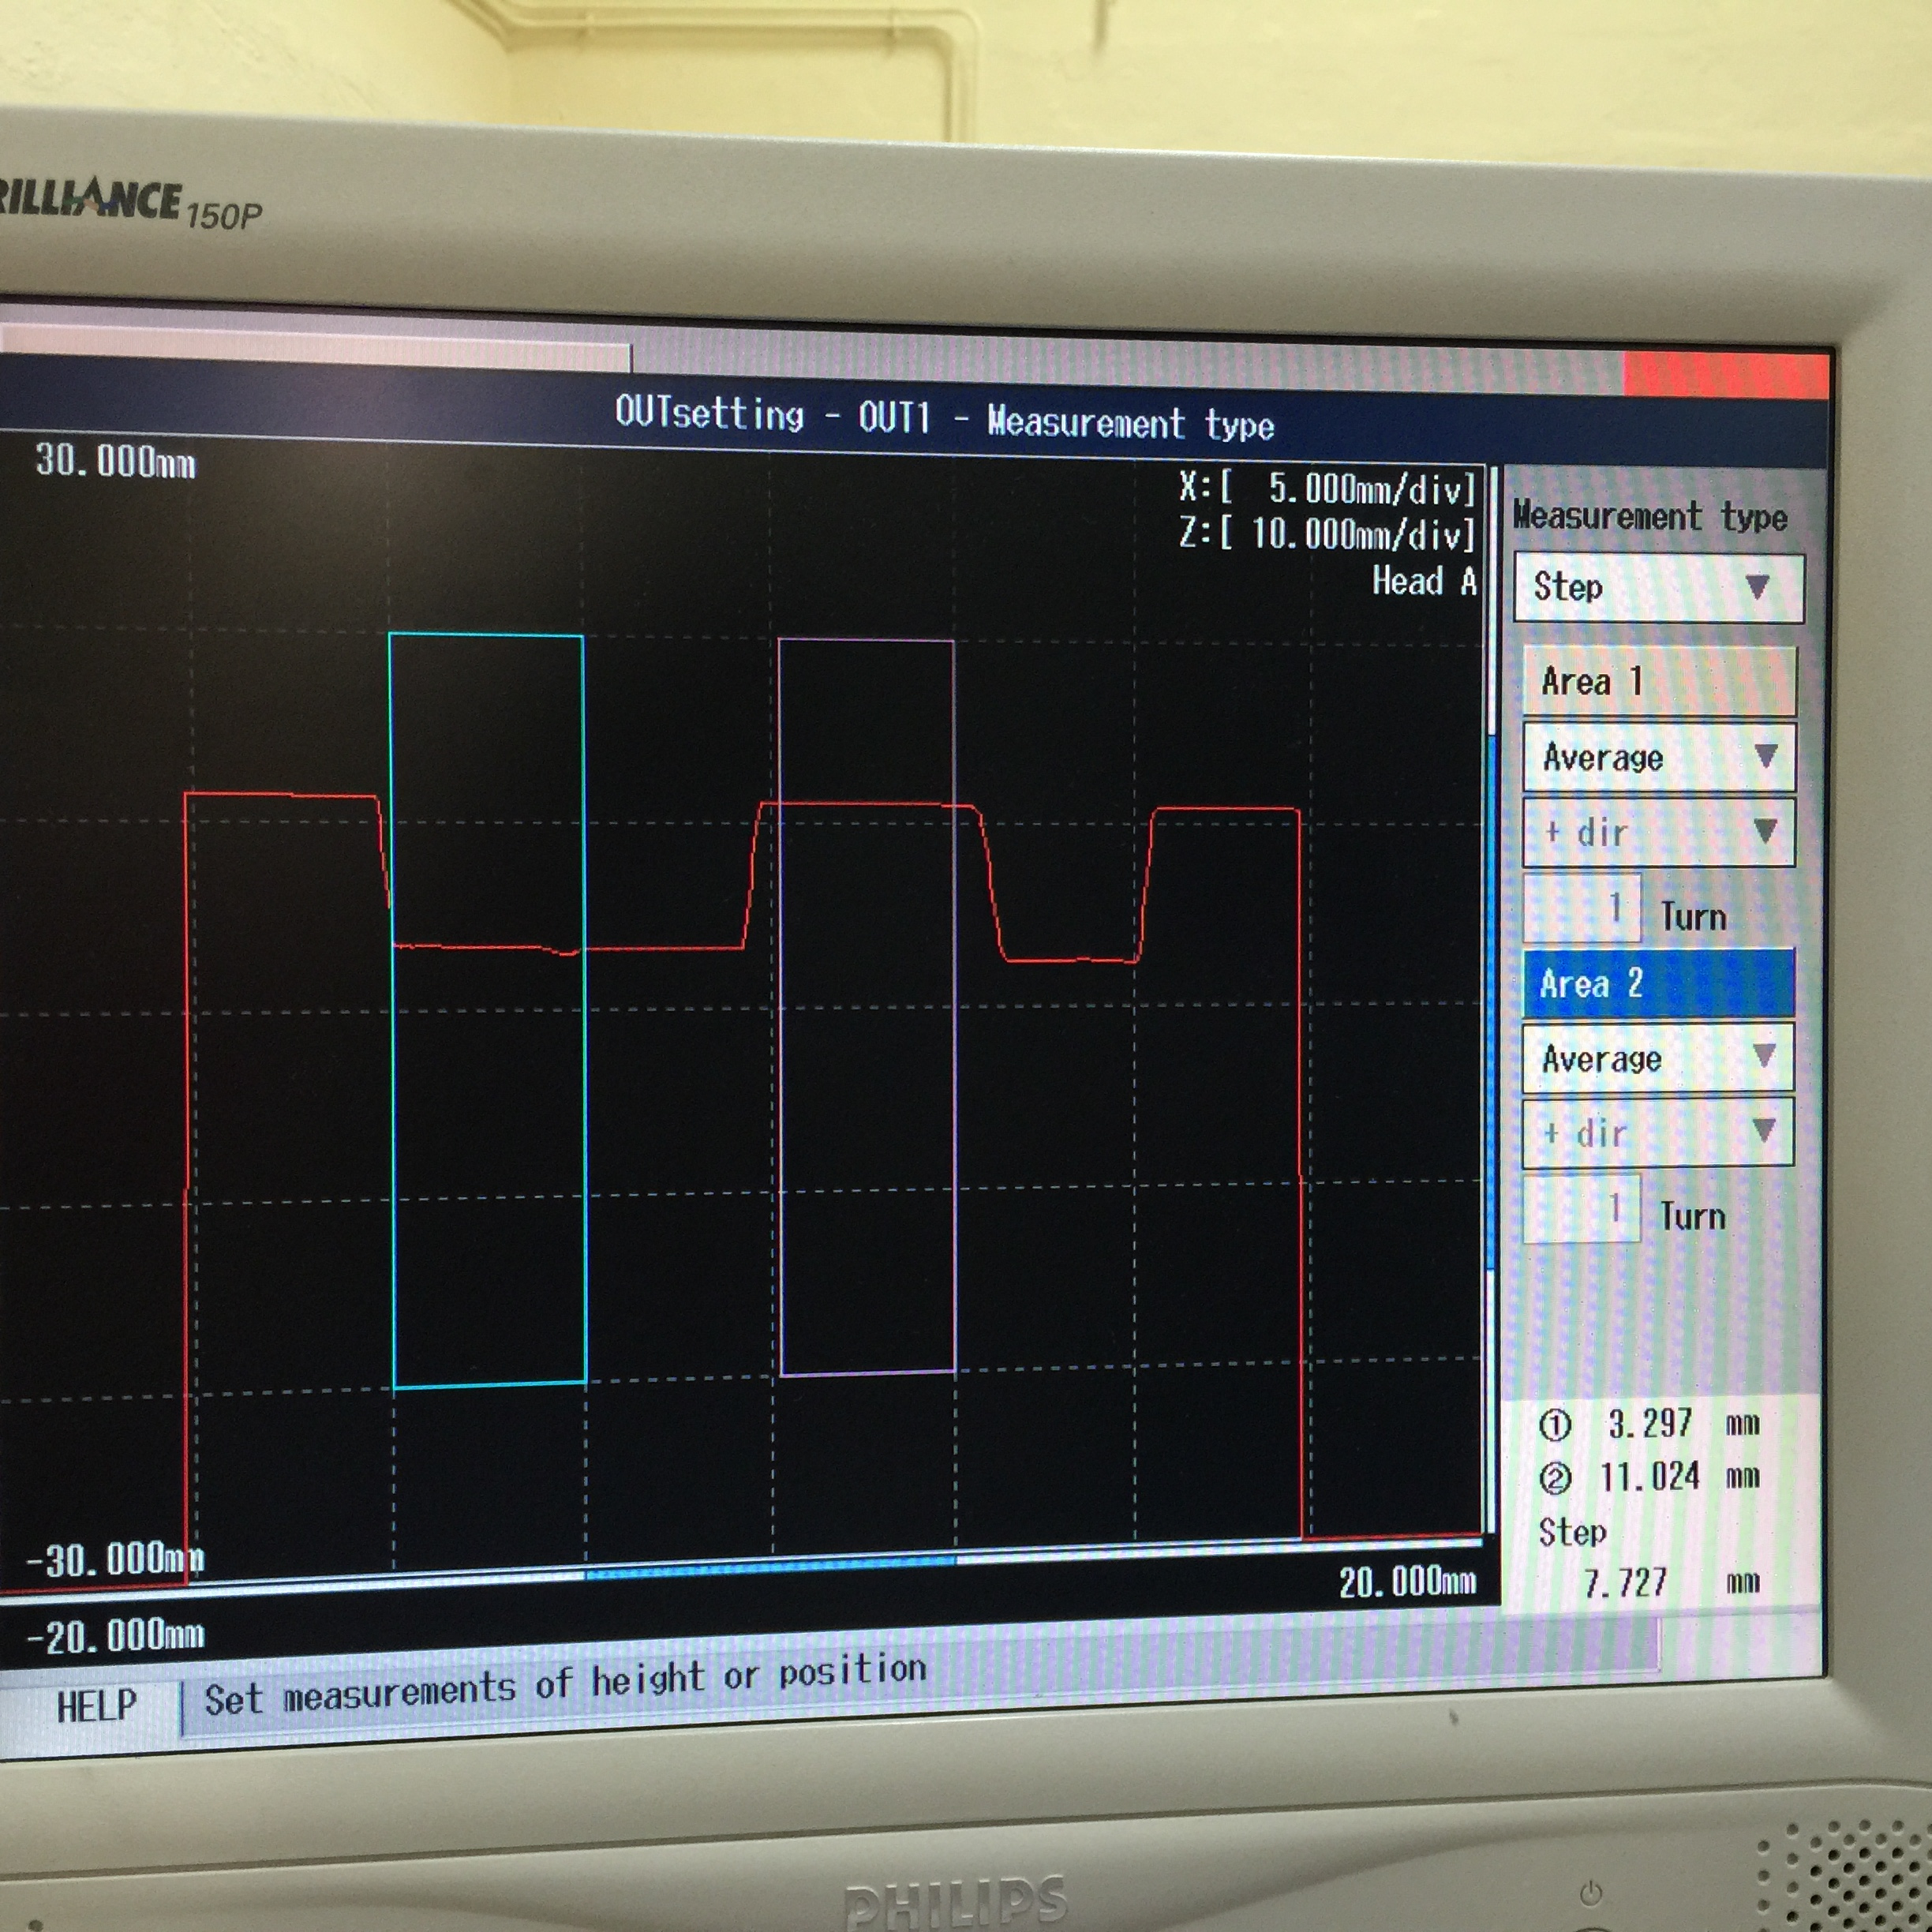
\includegraphics[width=0.8\linewidth]{Lab6/Step1.JPG}
	\caption{Set regions of interest in order to measure the height}
	\label{fig:one}
\end{figure}

After height is measured, we starts to consider what if the object is shifted and angle is changed. So we perform shift and angle correction by setting region of moving in the "Pos corr". The height numbers in the up right side of Figure \ref{fig:twoa} and Figure \ref{fig:twob} show that, accurate measured height could still be acquired even the object is shifted or rotated.\\

\begin{figure}[H]
	\centering
	\subfigure[Original]{\label{fig:twoa}
	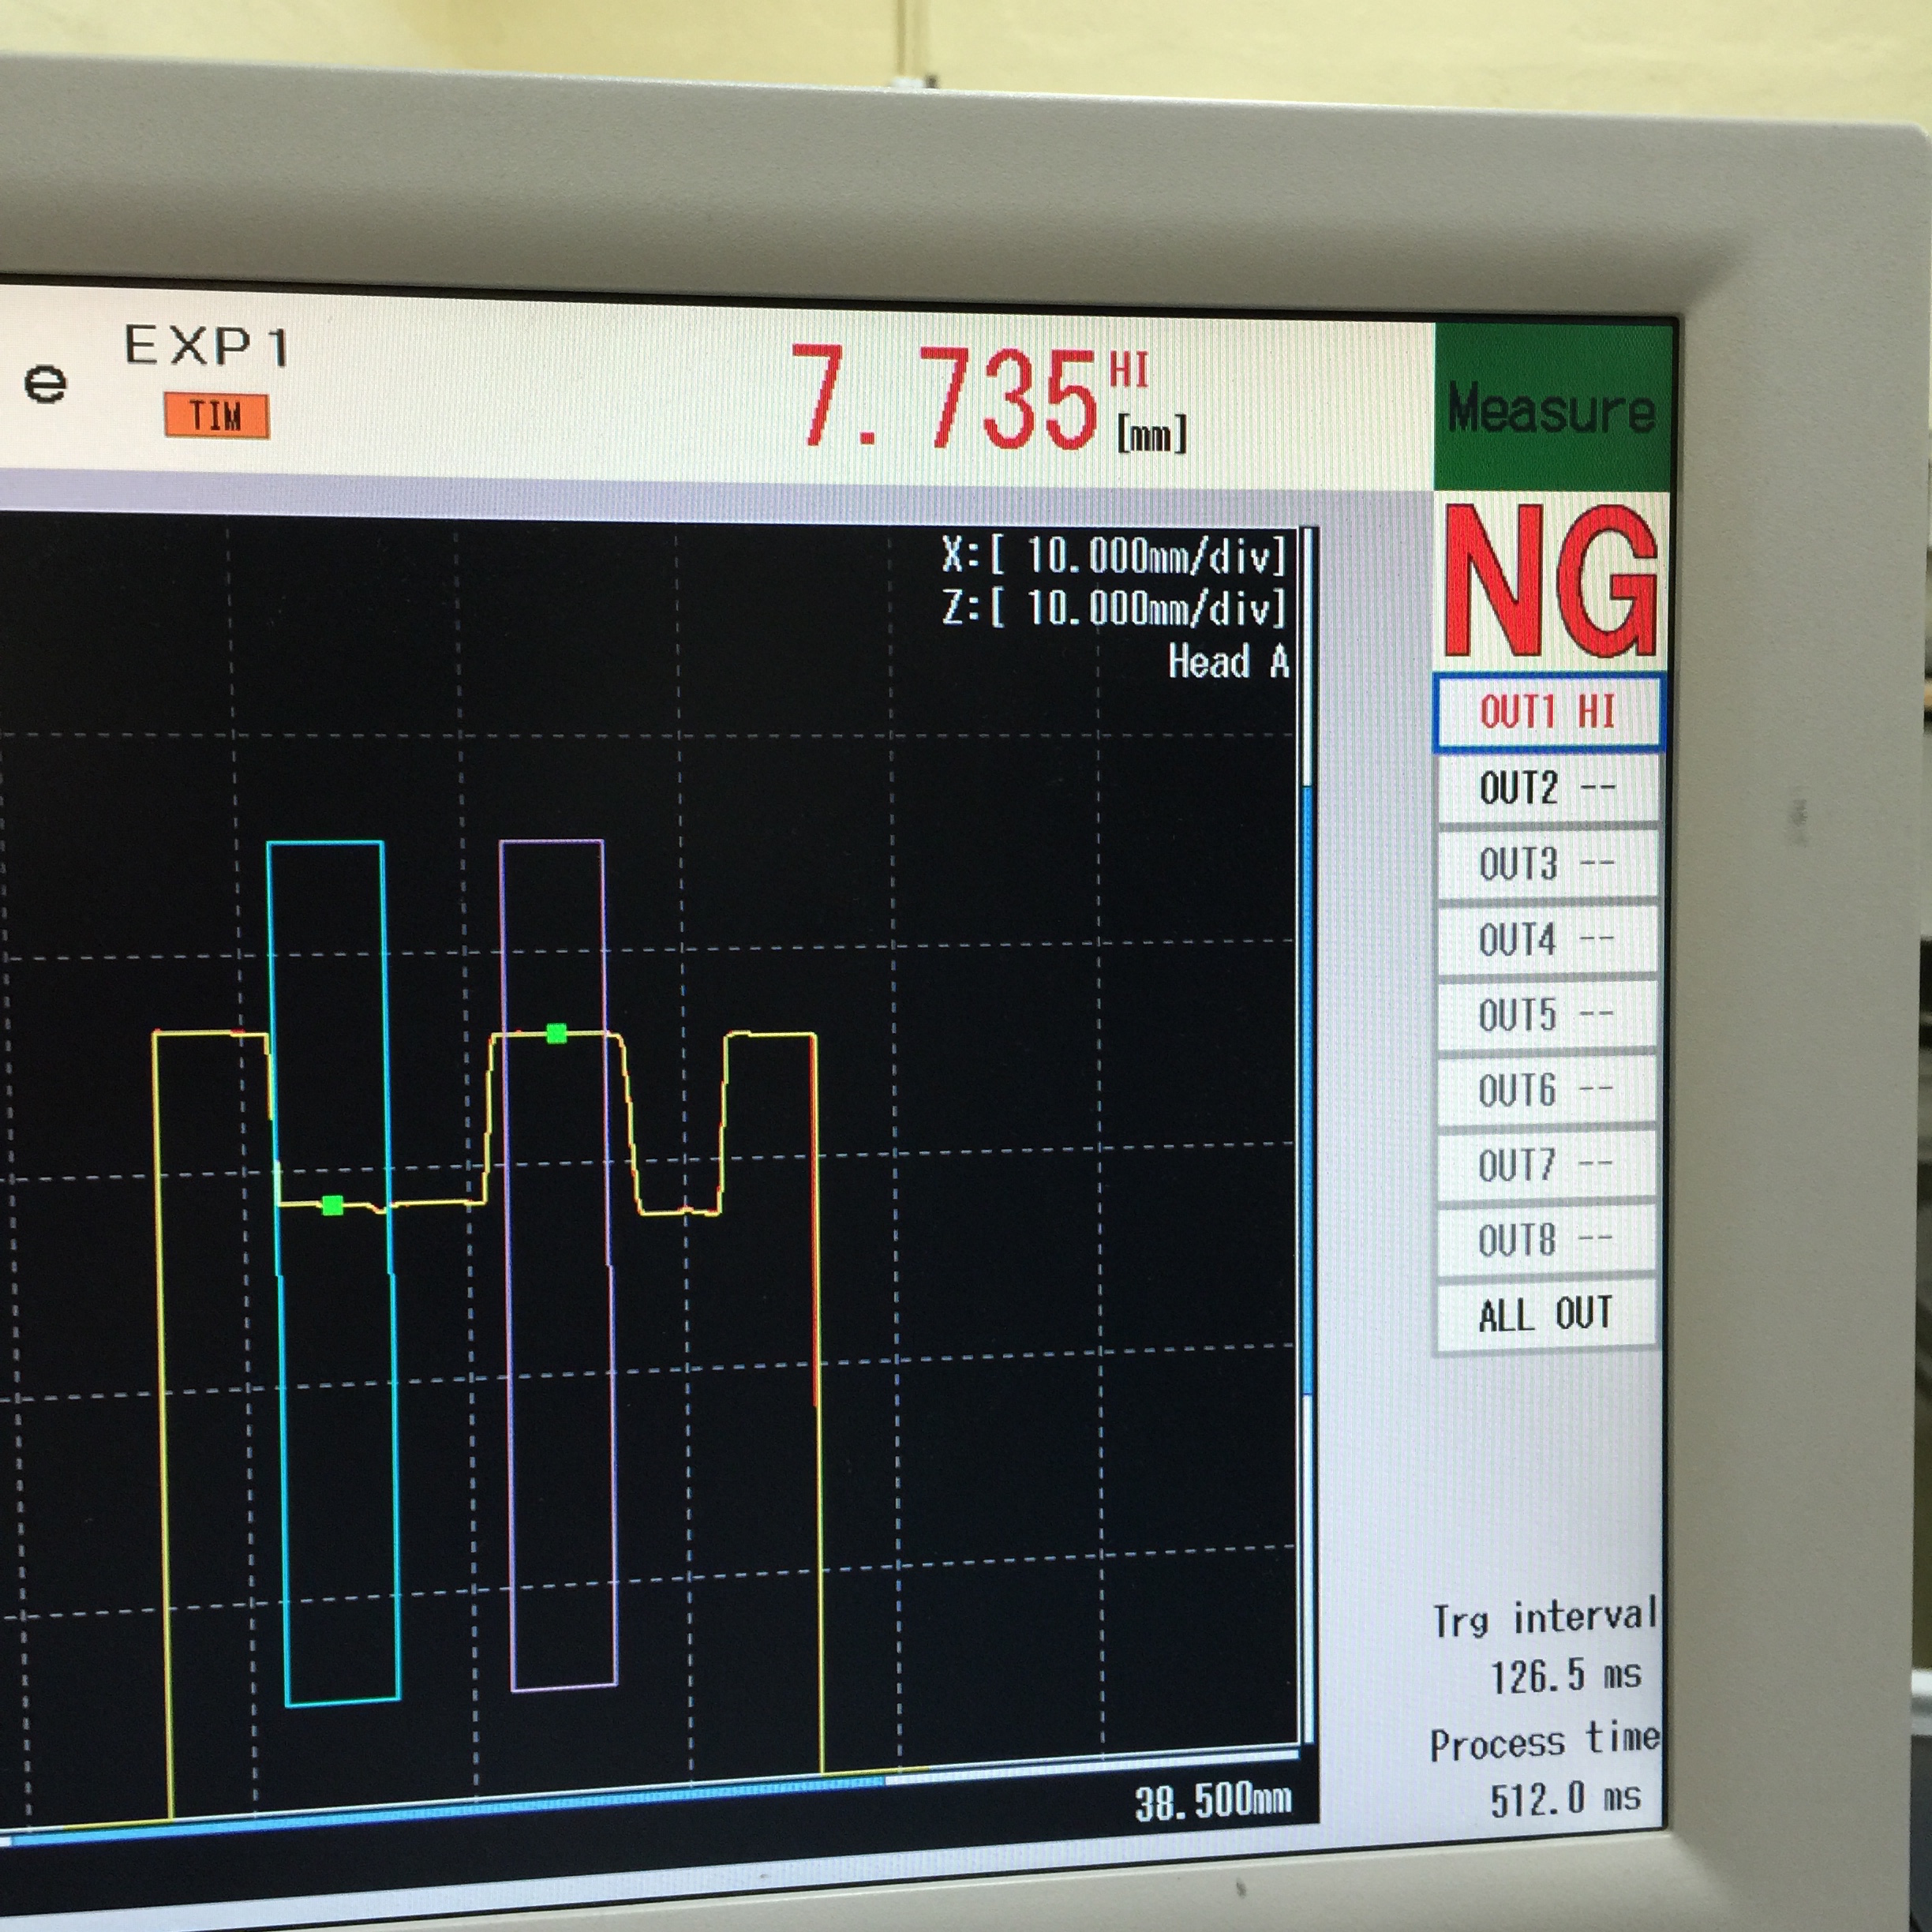
\includegraphics[width=0.4\linewidth]{Lab6/Step2.JPG}
	}
	\subfigure[Shift and Angle]{\label{fig:twob}
	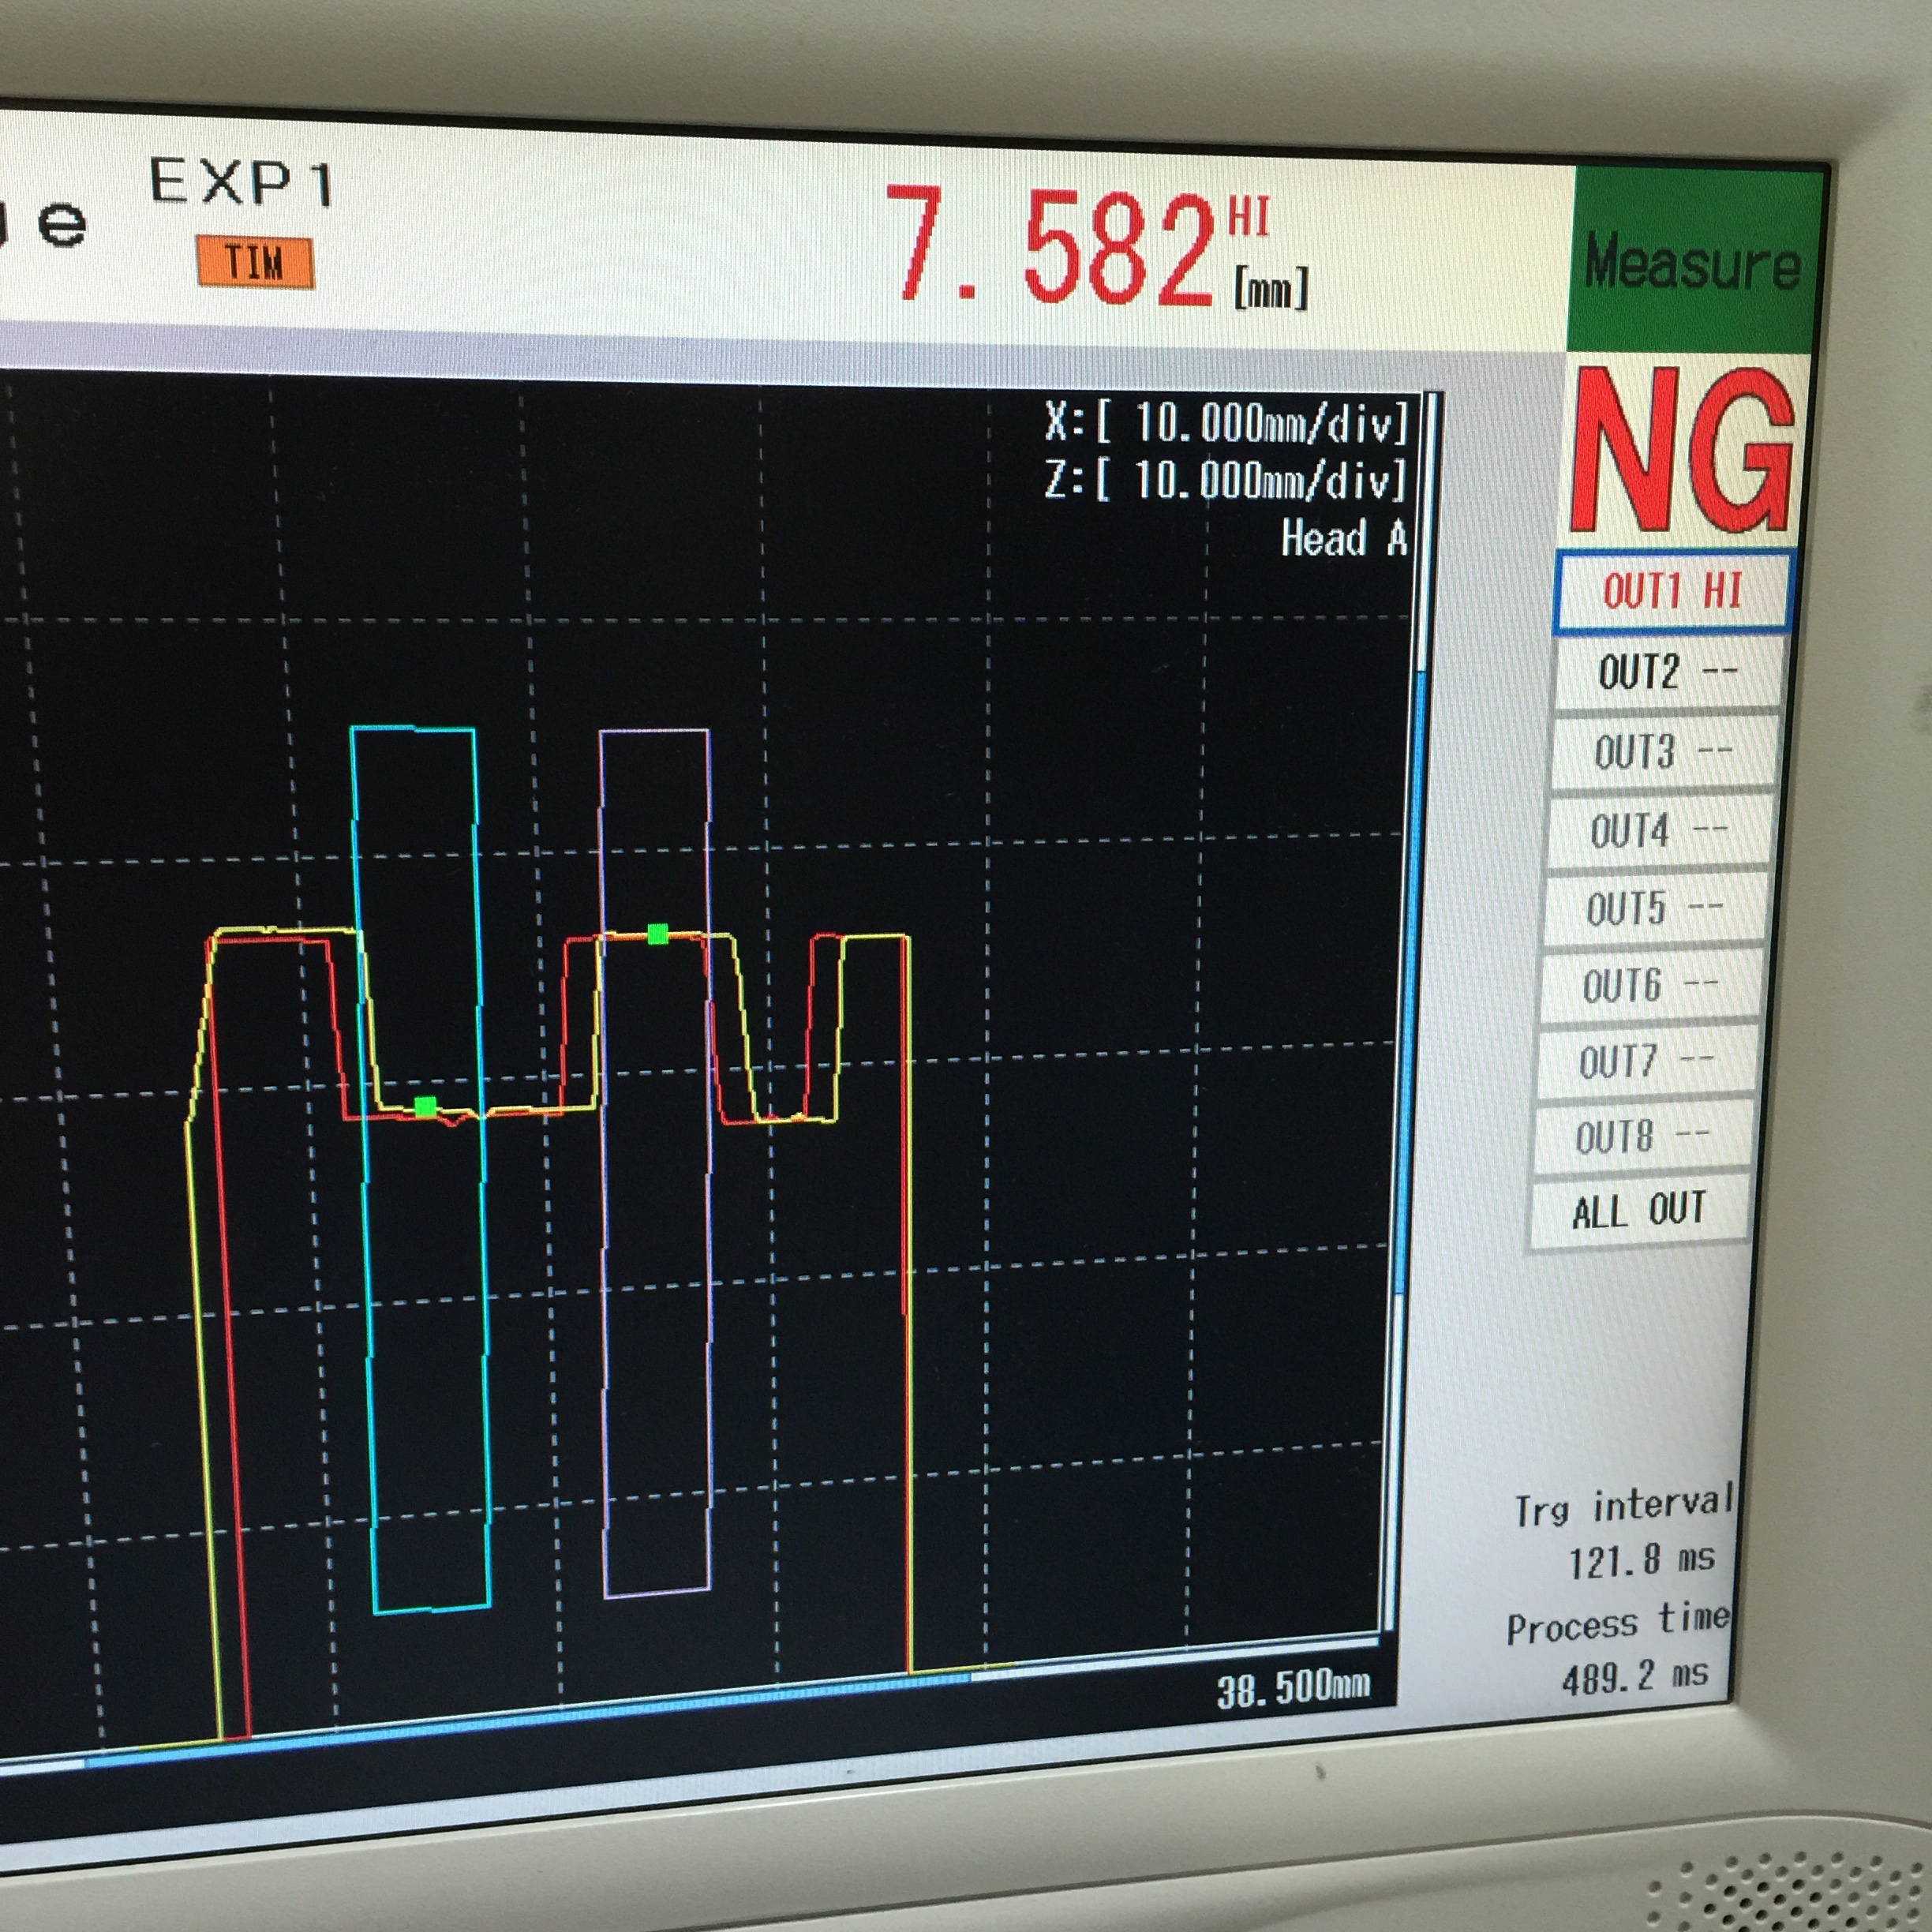
\includegraphics[width=0.4\linewidth]{Lab6/Step4.JPG}
	}
	\caption{Position correlation for Step measurement}
	\label{fig:two}
\end{figure}

\section*{Angle Measurement on Shiny Surface}
In this part, we try to measure the angle of an object with shiny surface and several small holes, shown in Figure \ref {fig:three}. \\ 

\begin{figure}[H]
	\centering
	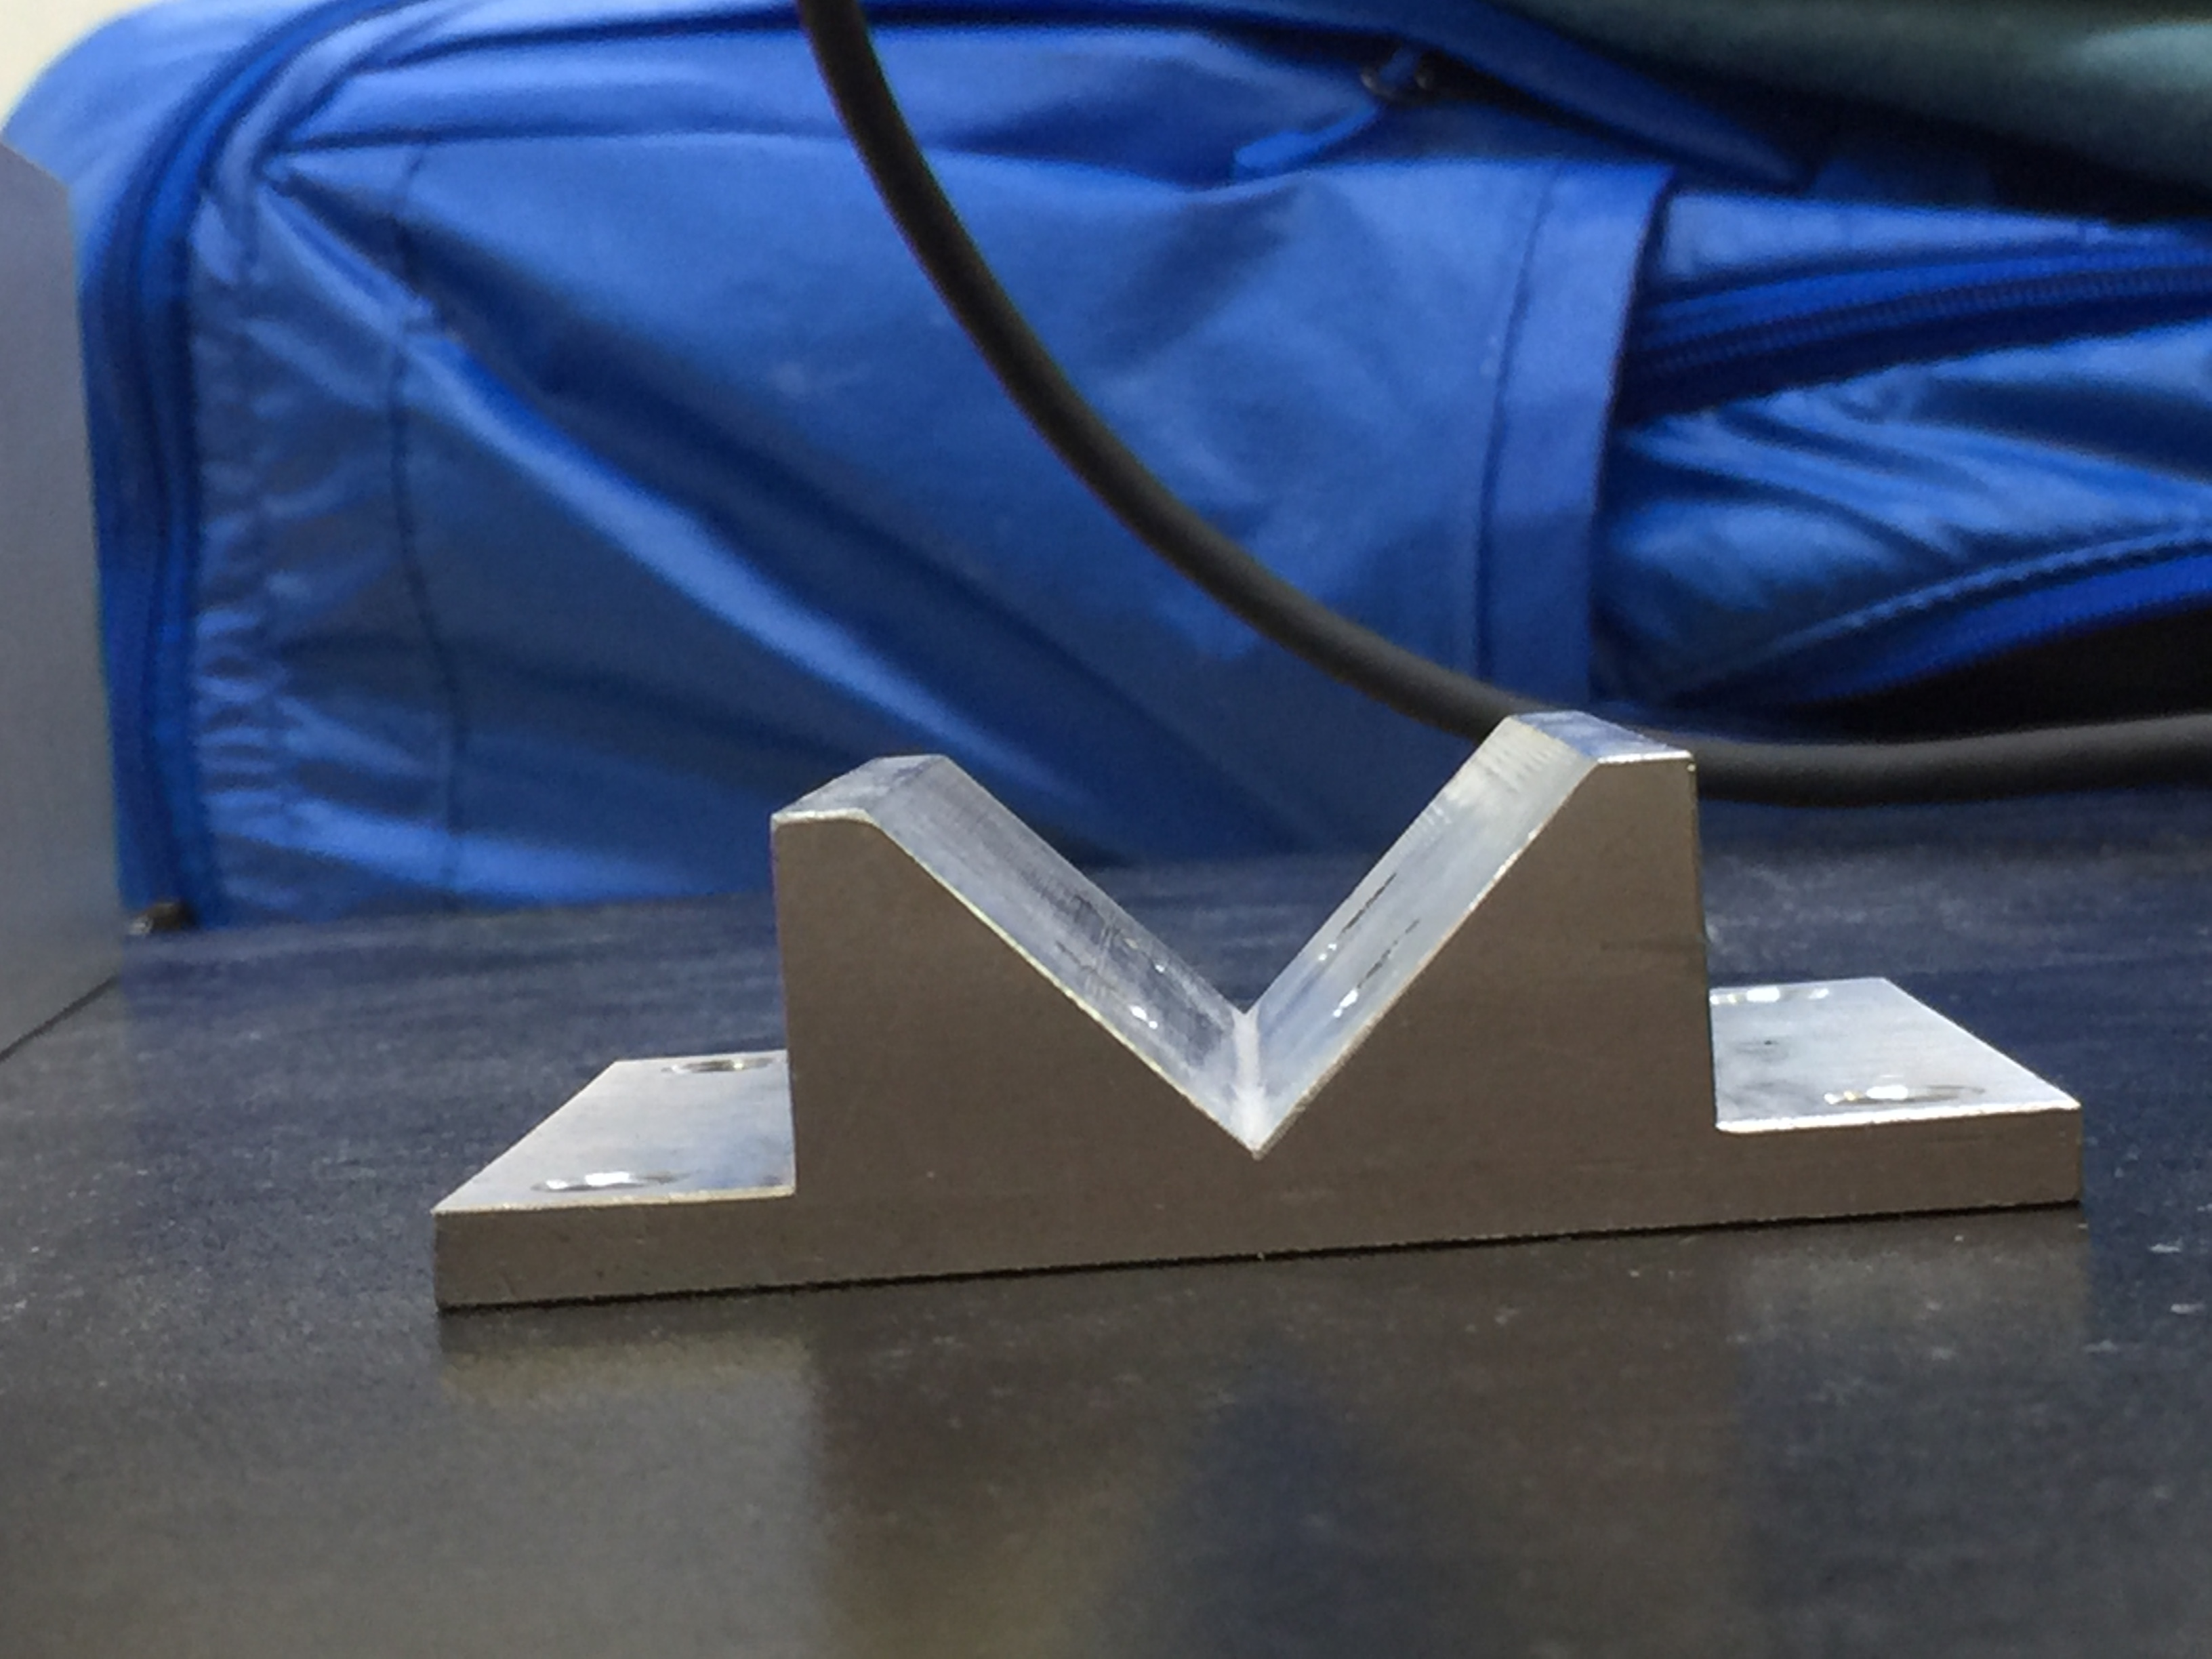
\includegraphics[width=0.8\linewidth]{Lab6/Angle5.JPG}
	\caption{Object with shiny surface}
	\label{fig:three}
\end{figure}

In order to characterize the angle between two planes, similarly, we should first adjust camera to a proper height so that we can get profile of the object. Then use "Master reg" to keep the profile. Finally, the measurement type in "OUT setting" should be set to "Angle" and the regions of interest are also adjusted to a proper position, illustrated in Figure \ref{fig:four}. And the angle can be easily measured from the regions of interest.\\

\begin{figure}[H]
	\centering
	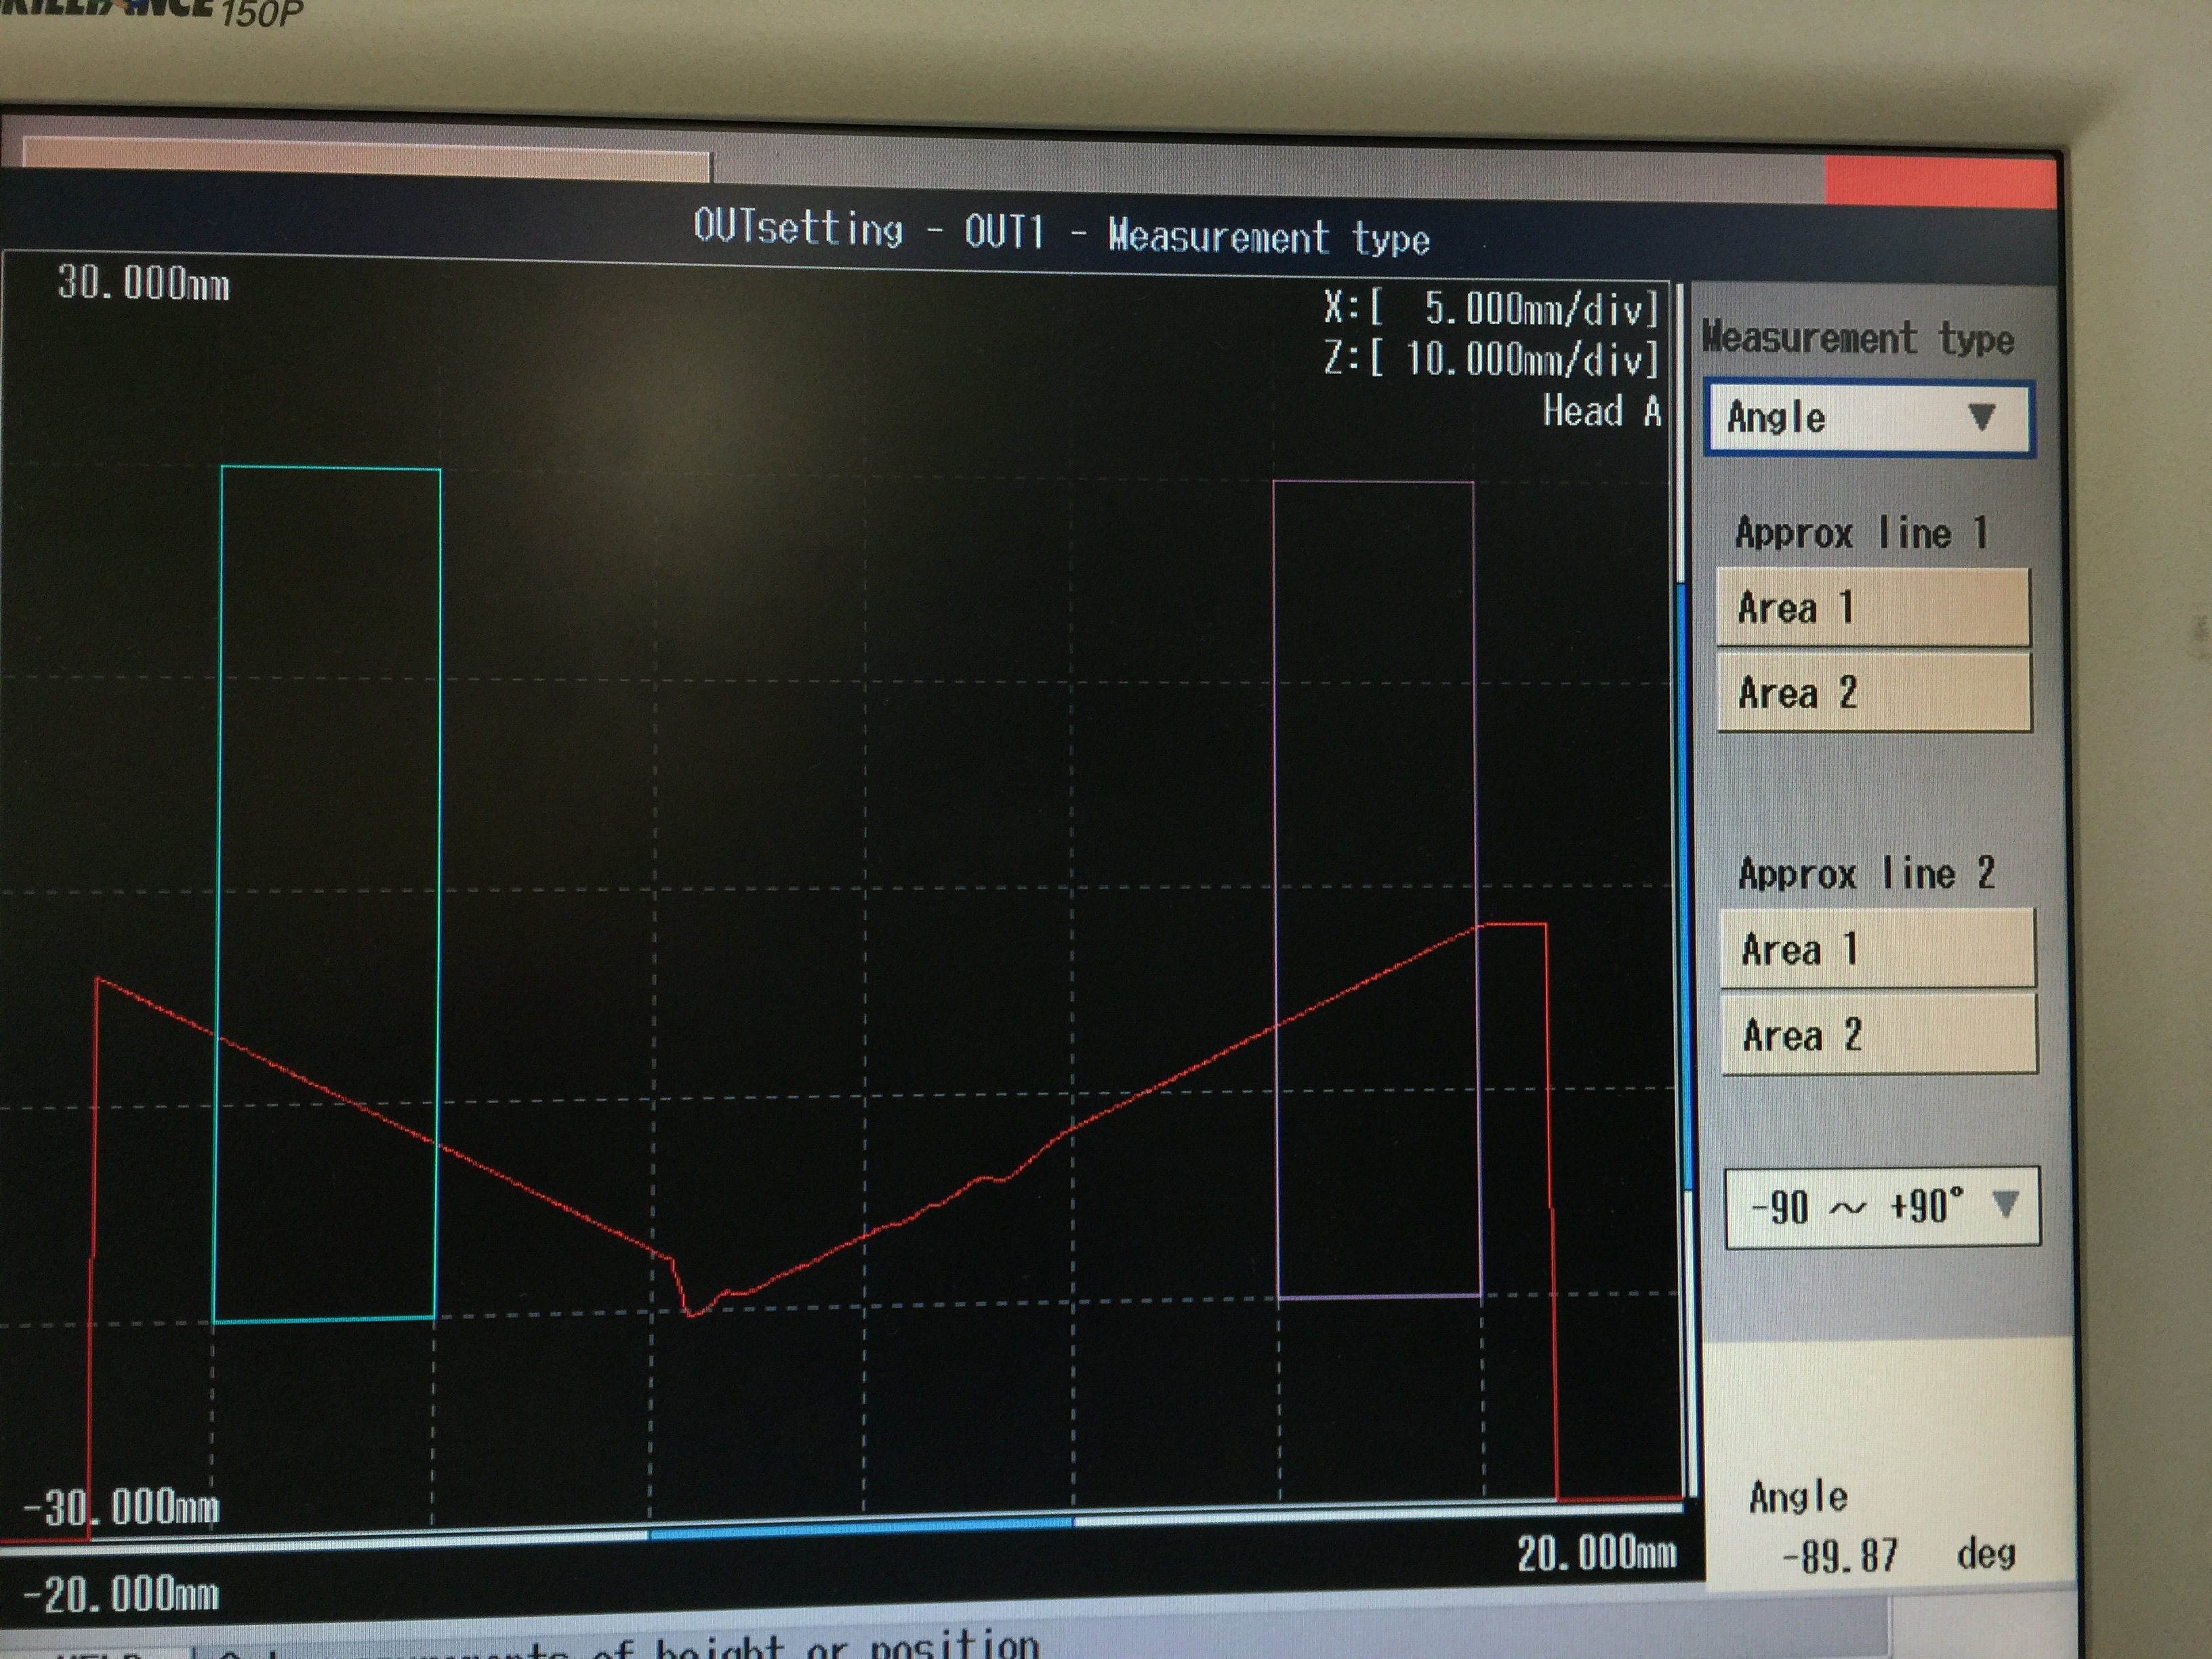
\includegraphics[width=0.8\linewidth]{Lab6/Angle1.JPG}
	\caption{Profile and regions of interest of object}
	\label{fig:four}
\end{figure}

Naturally, we want to enhance the measurement by position adjustment. After doing the similar thing as the last part, we get the result. Figure \ref{fig:fivea} and Figure \ref{fig:fiveb} are two measurements when the object is shifted or rotated in two different way. It turns out that both outcomes can give us a really good measurement.

\begin{figure}[H]
	\centering
	\subfigure[Original]{\label{fig:fivea}
	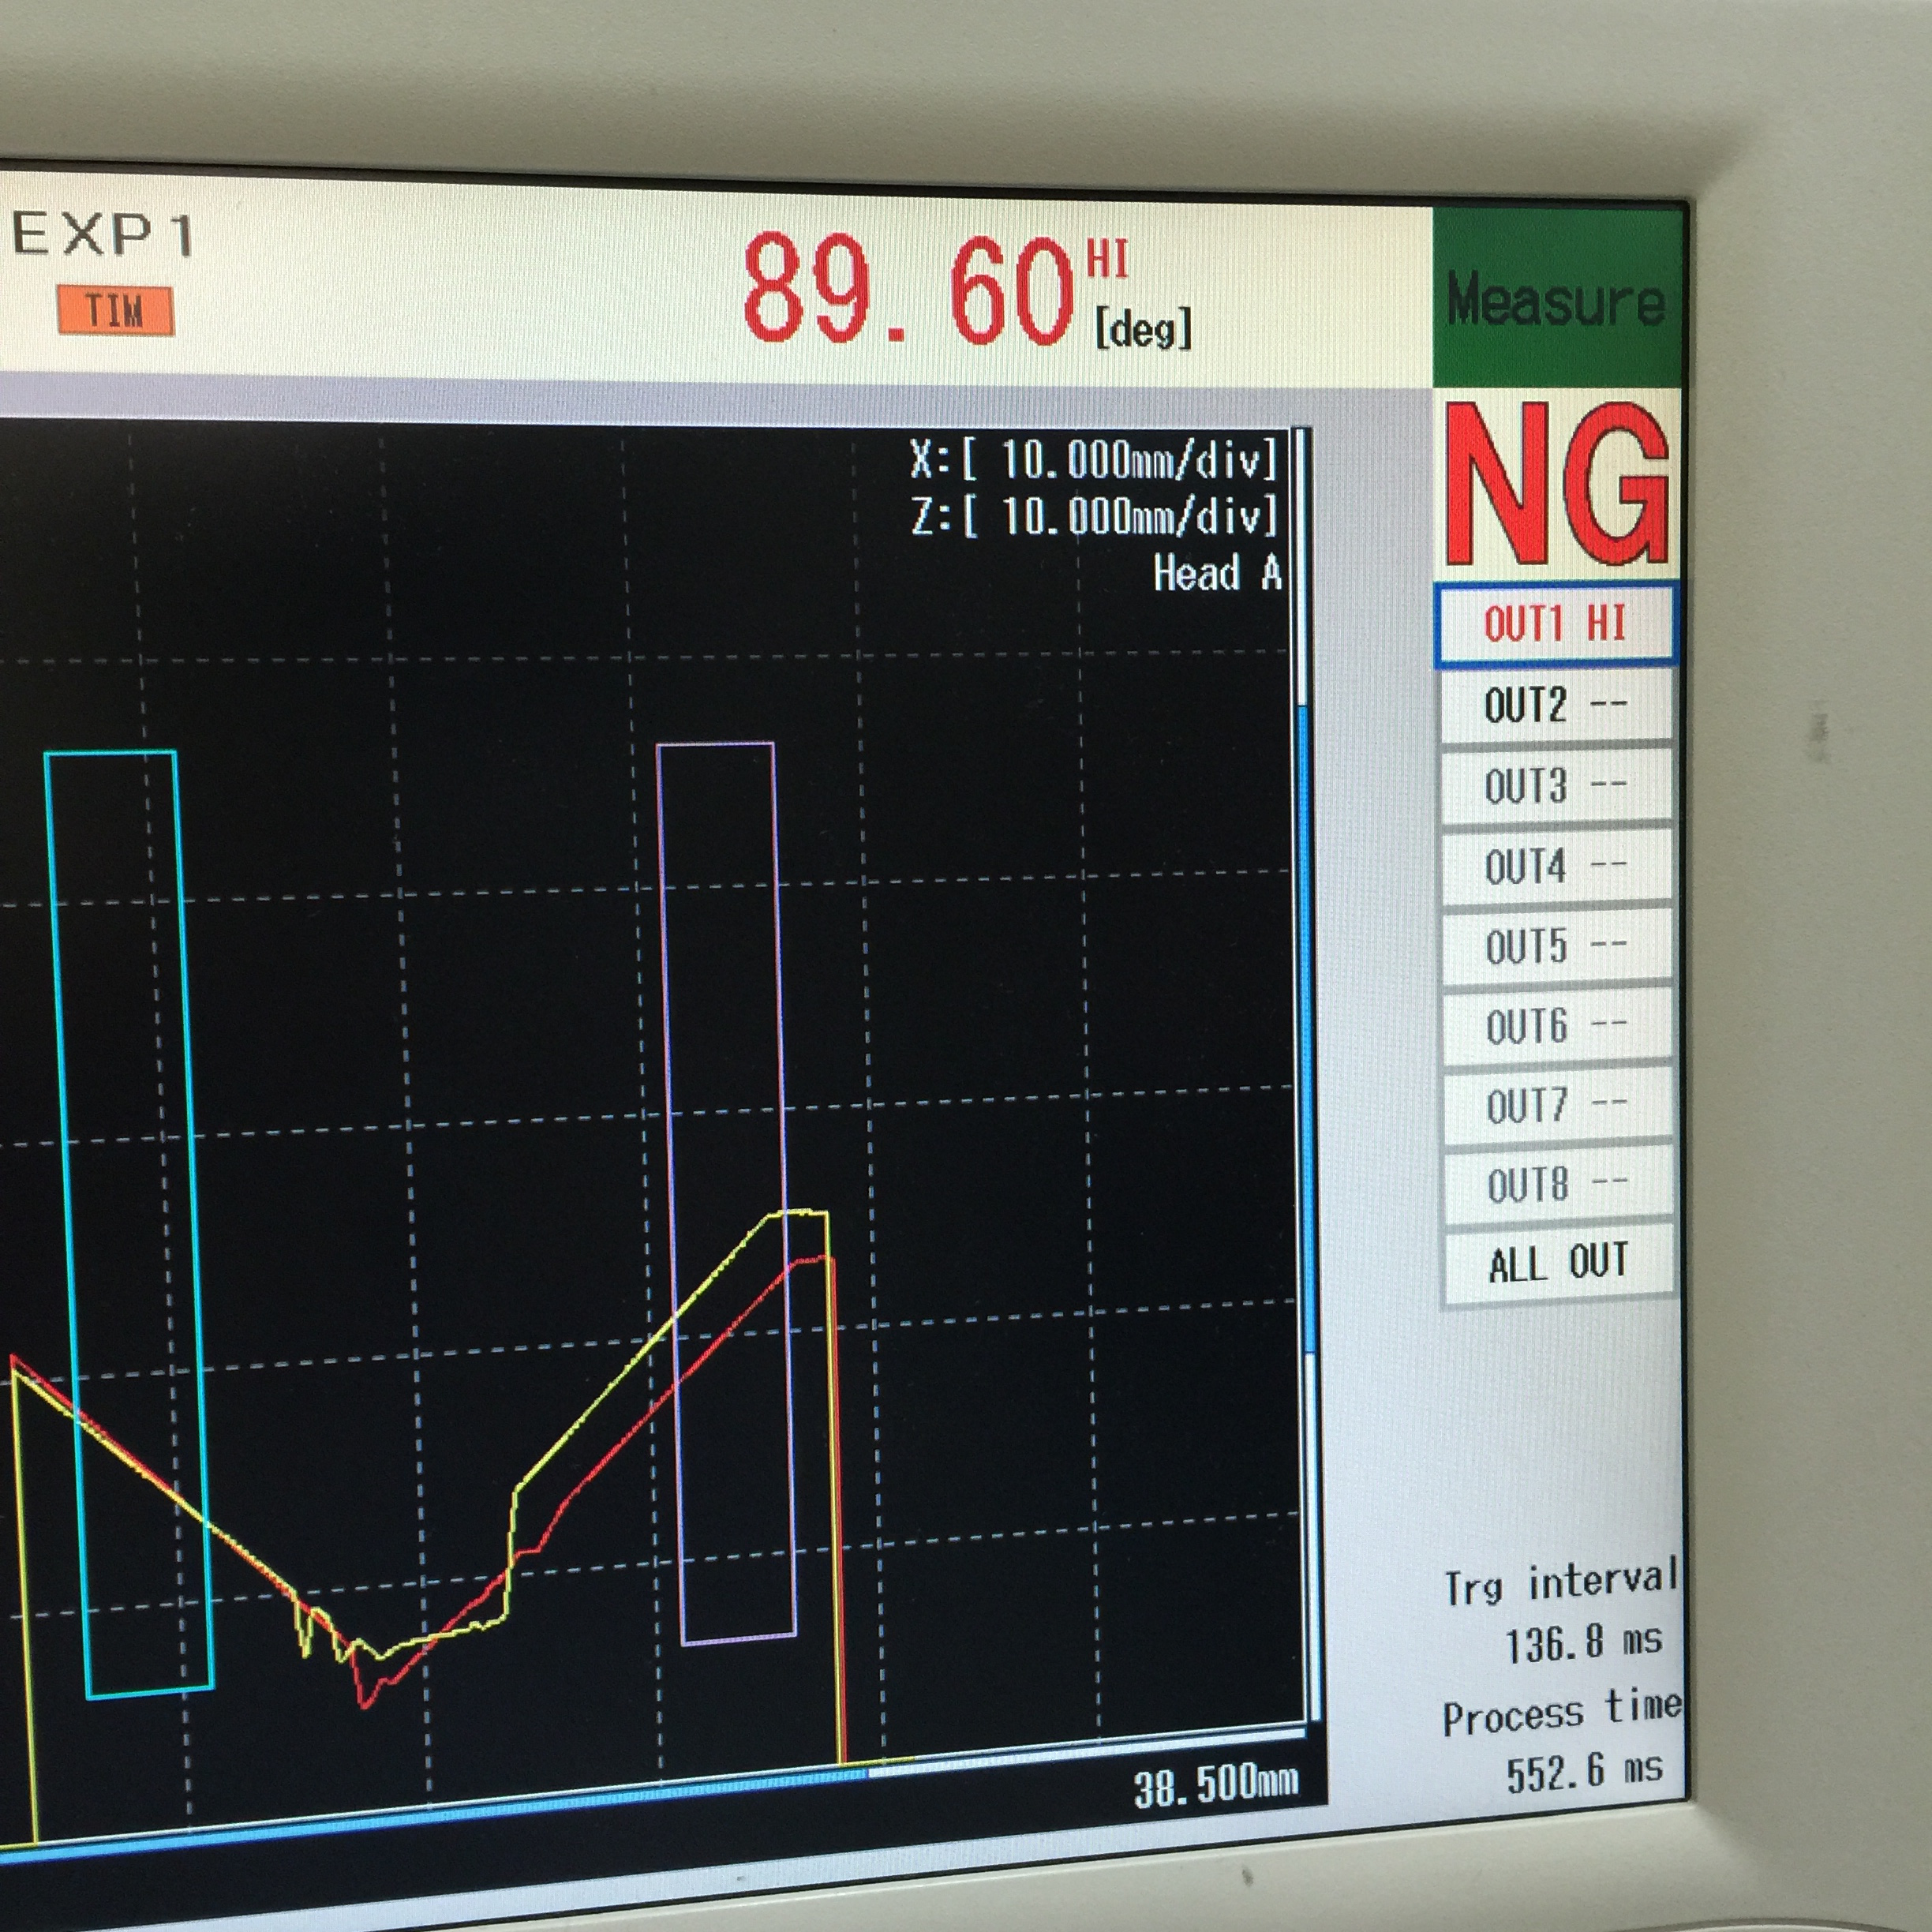
\includegraphics[width=0.4\linewidth]{Lab6/Angle3.JPG}
	}
	\subfigure[Shift and Angle]{\label{fig:fiveb}
	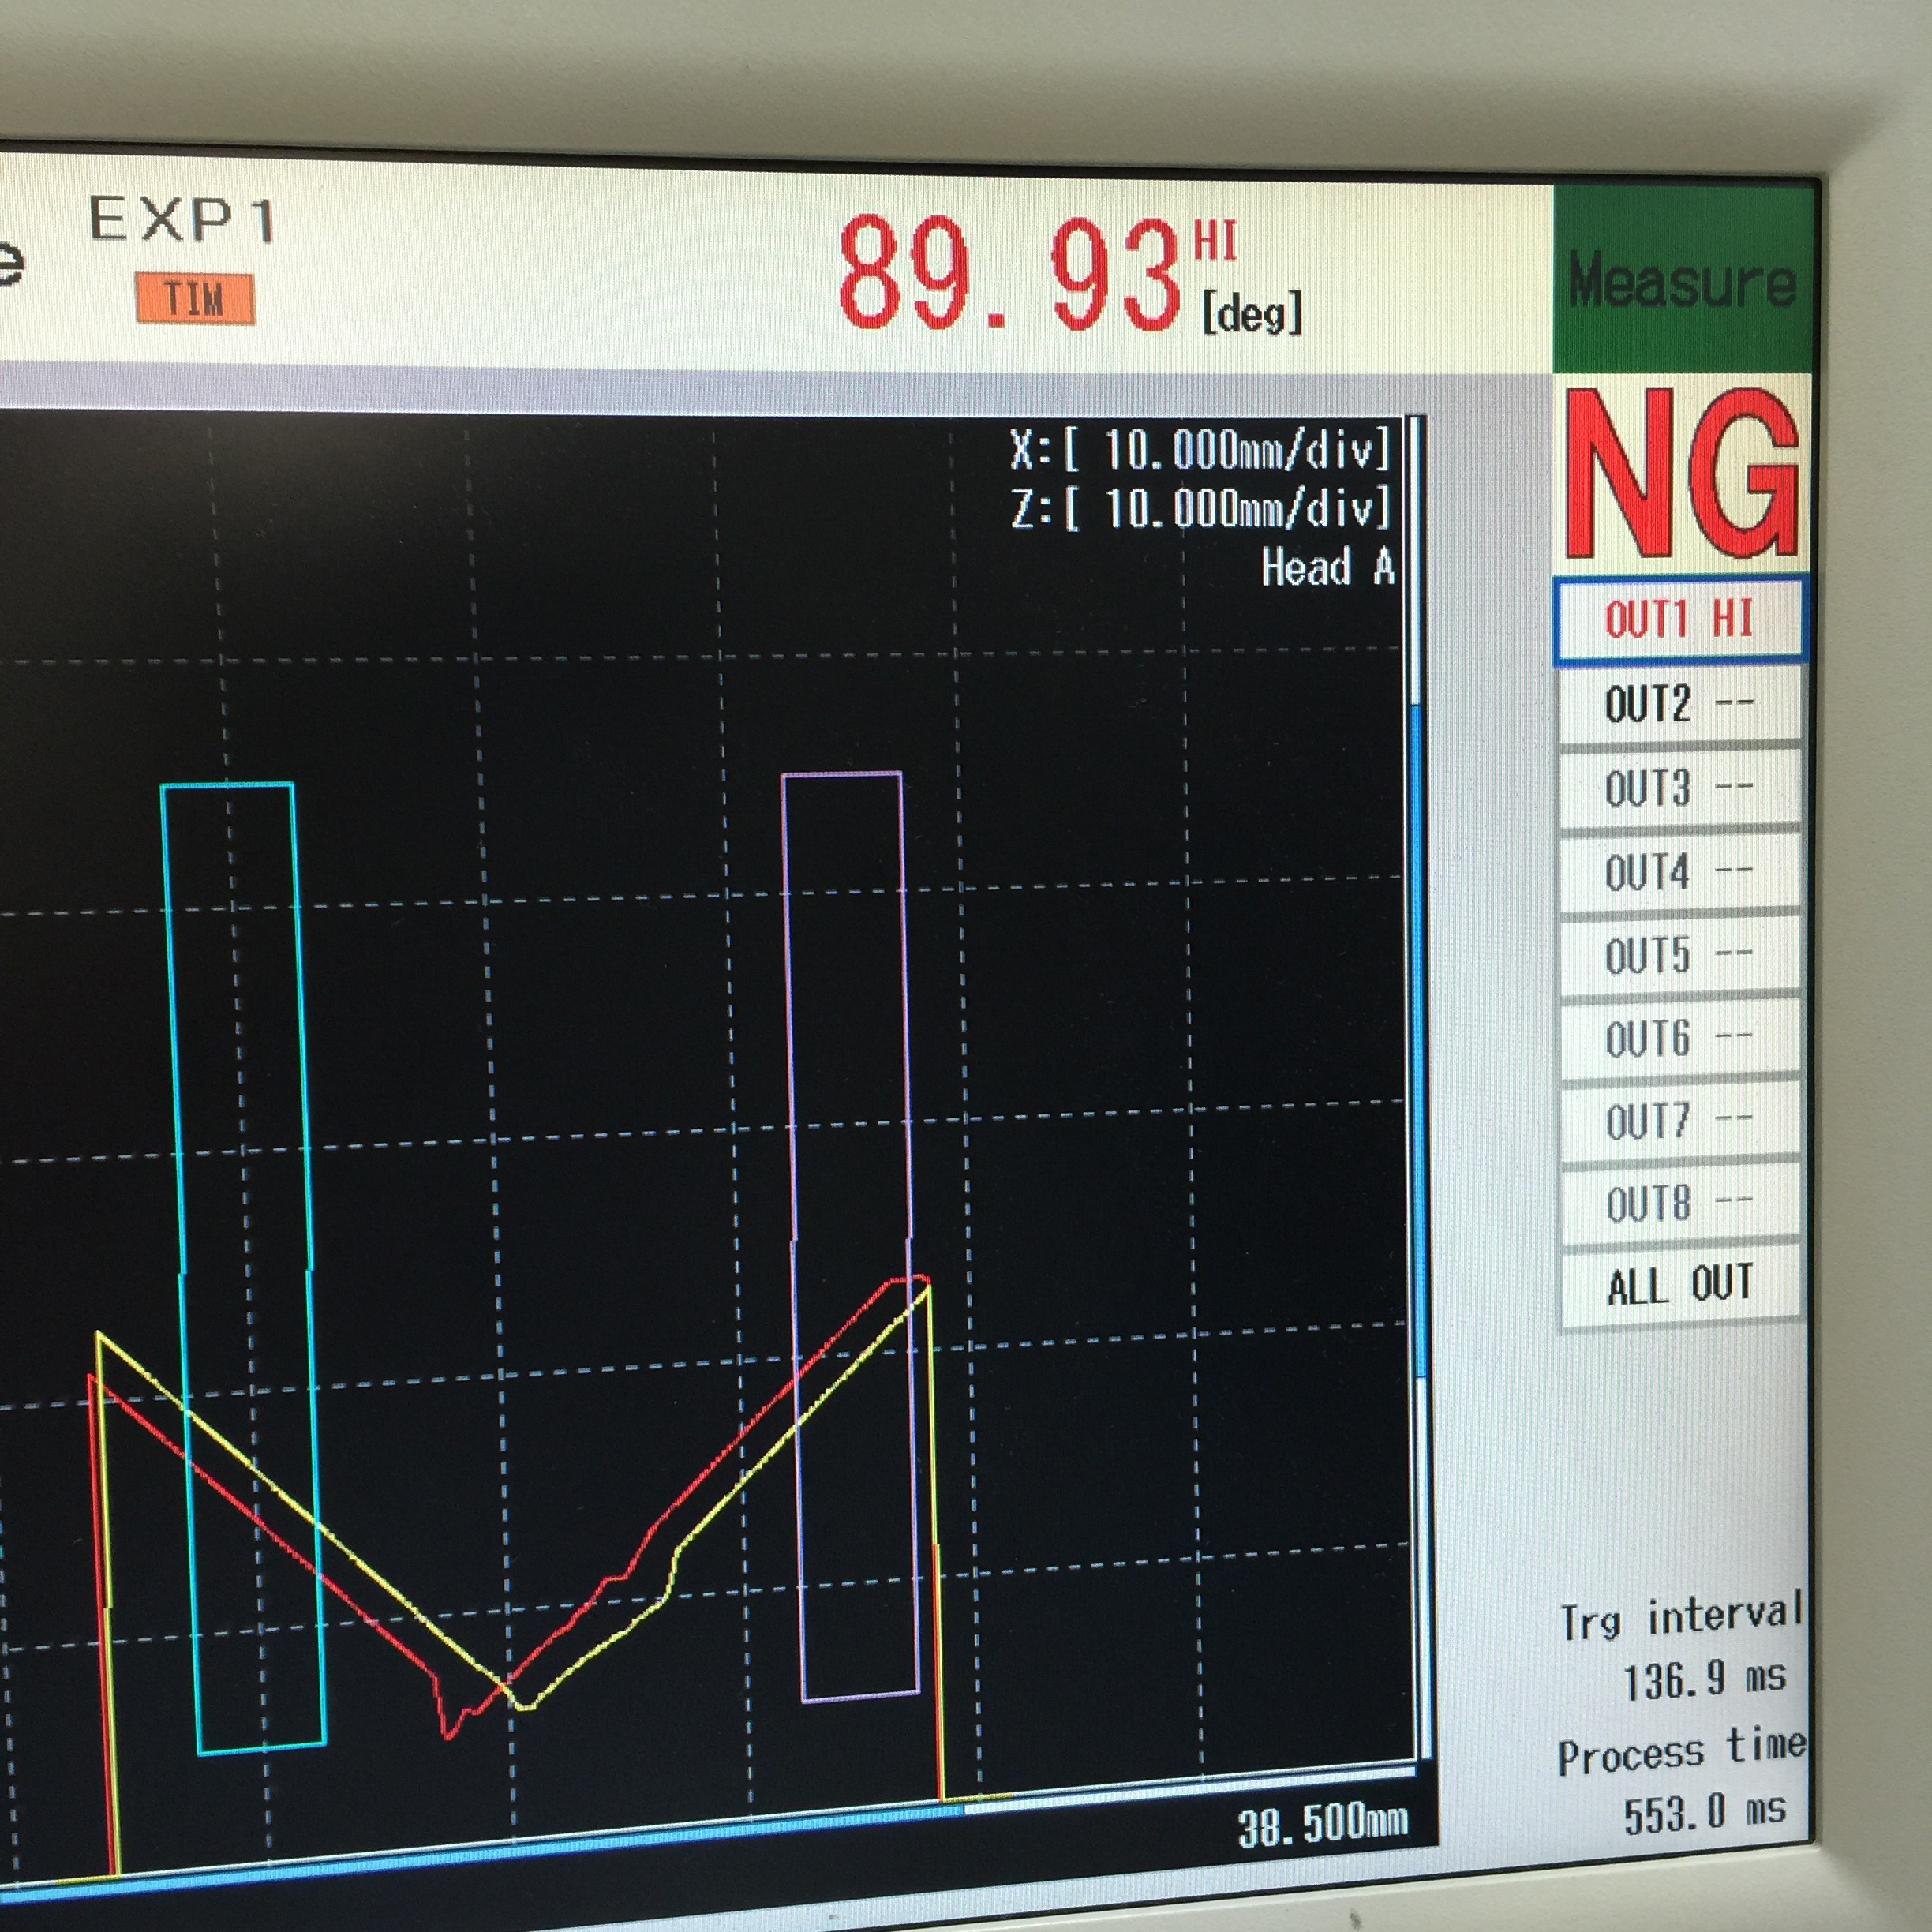
\includegraphics[width=0.4\linewidth]{Lab6/Angle4.JPG}
	}
	\caption{Measurement in different case of shift and rotation}
	\label{fig:five}
\end{figure}

Finally, in this part, we want to acquire the goal of hole detection. First, In Figure \ref{fig:sixa}, we can see there are different kinds of holes. And then, Figure \ref{fig:sixb} and Figure \ref{fig:sixc} reflect how holes in the images looks like int the measurement. 

\begin{figure}[H]
	\centering
	\subfigure[Holes in the object]{\label{fig:sixa}
	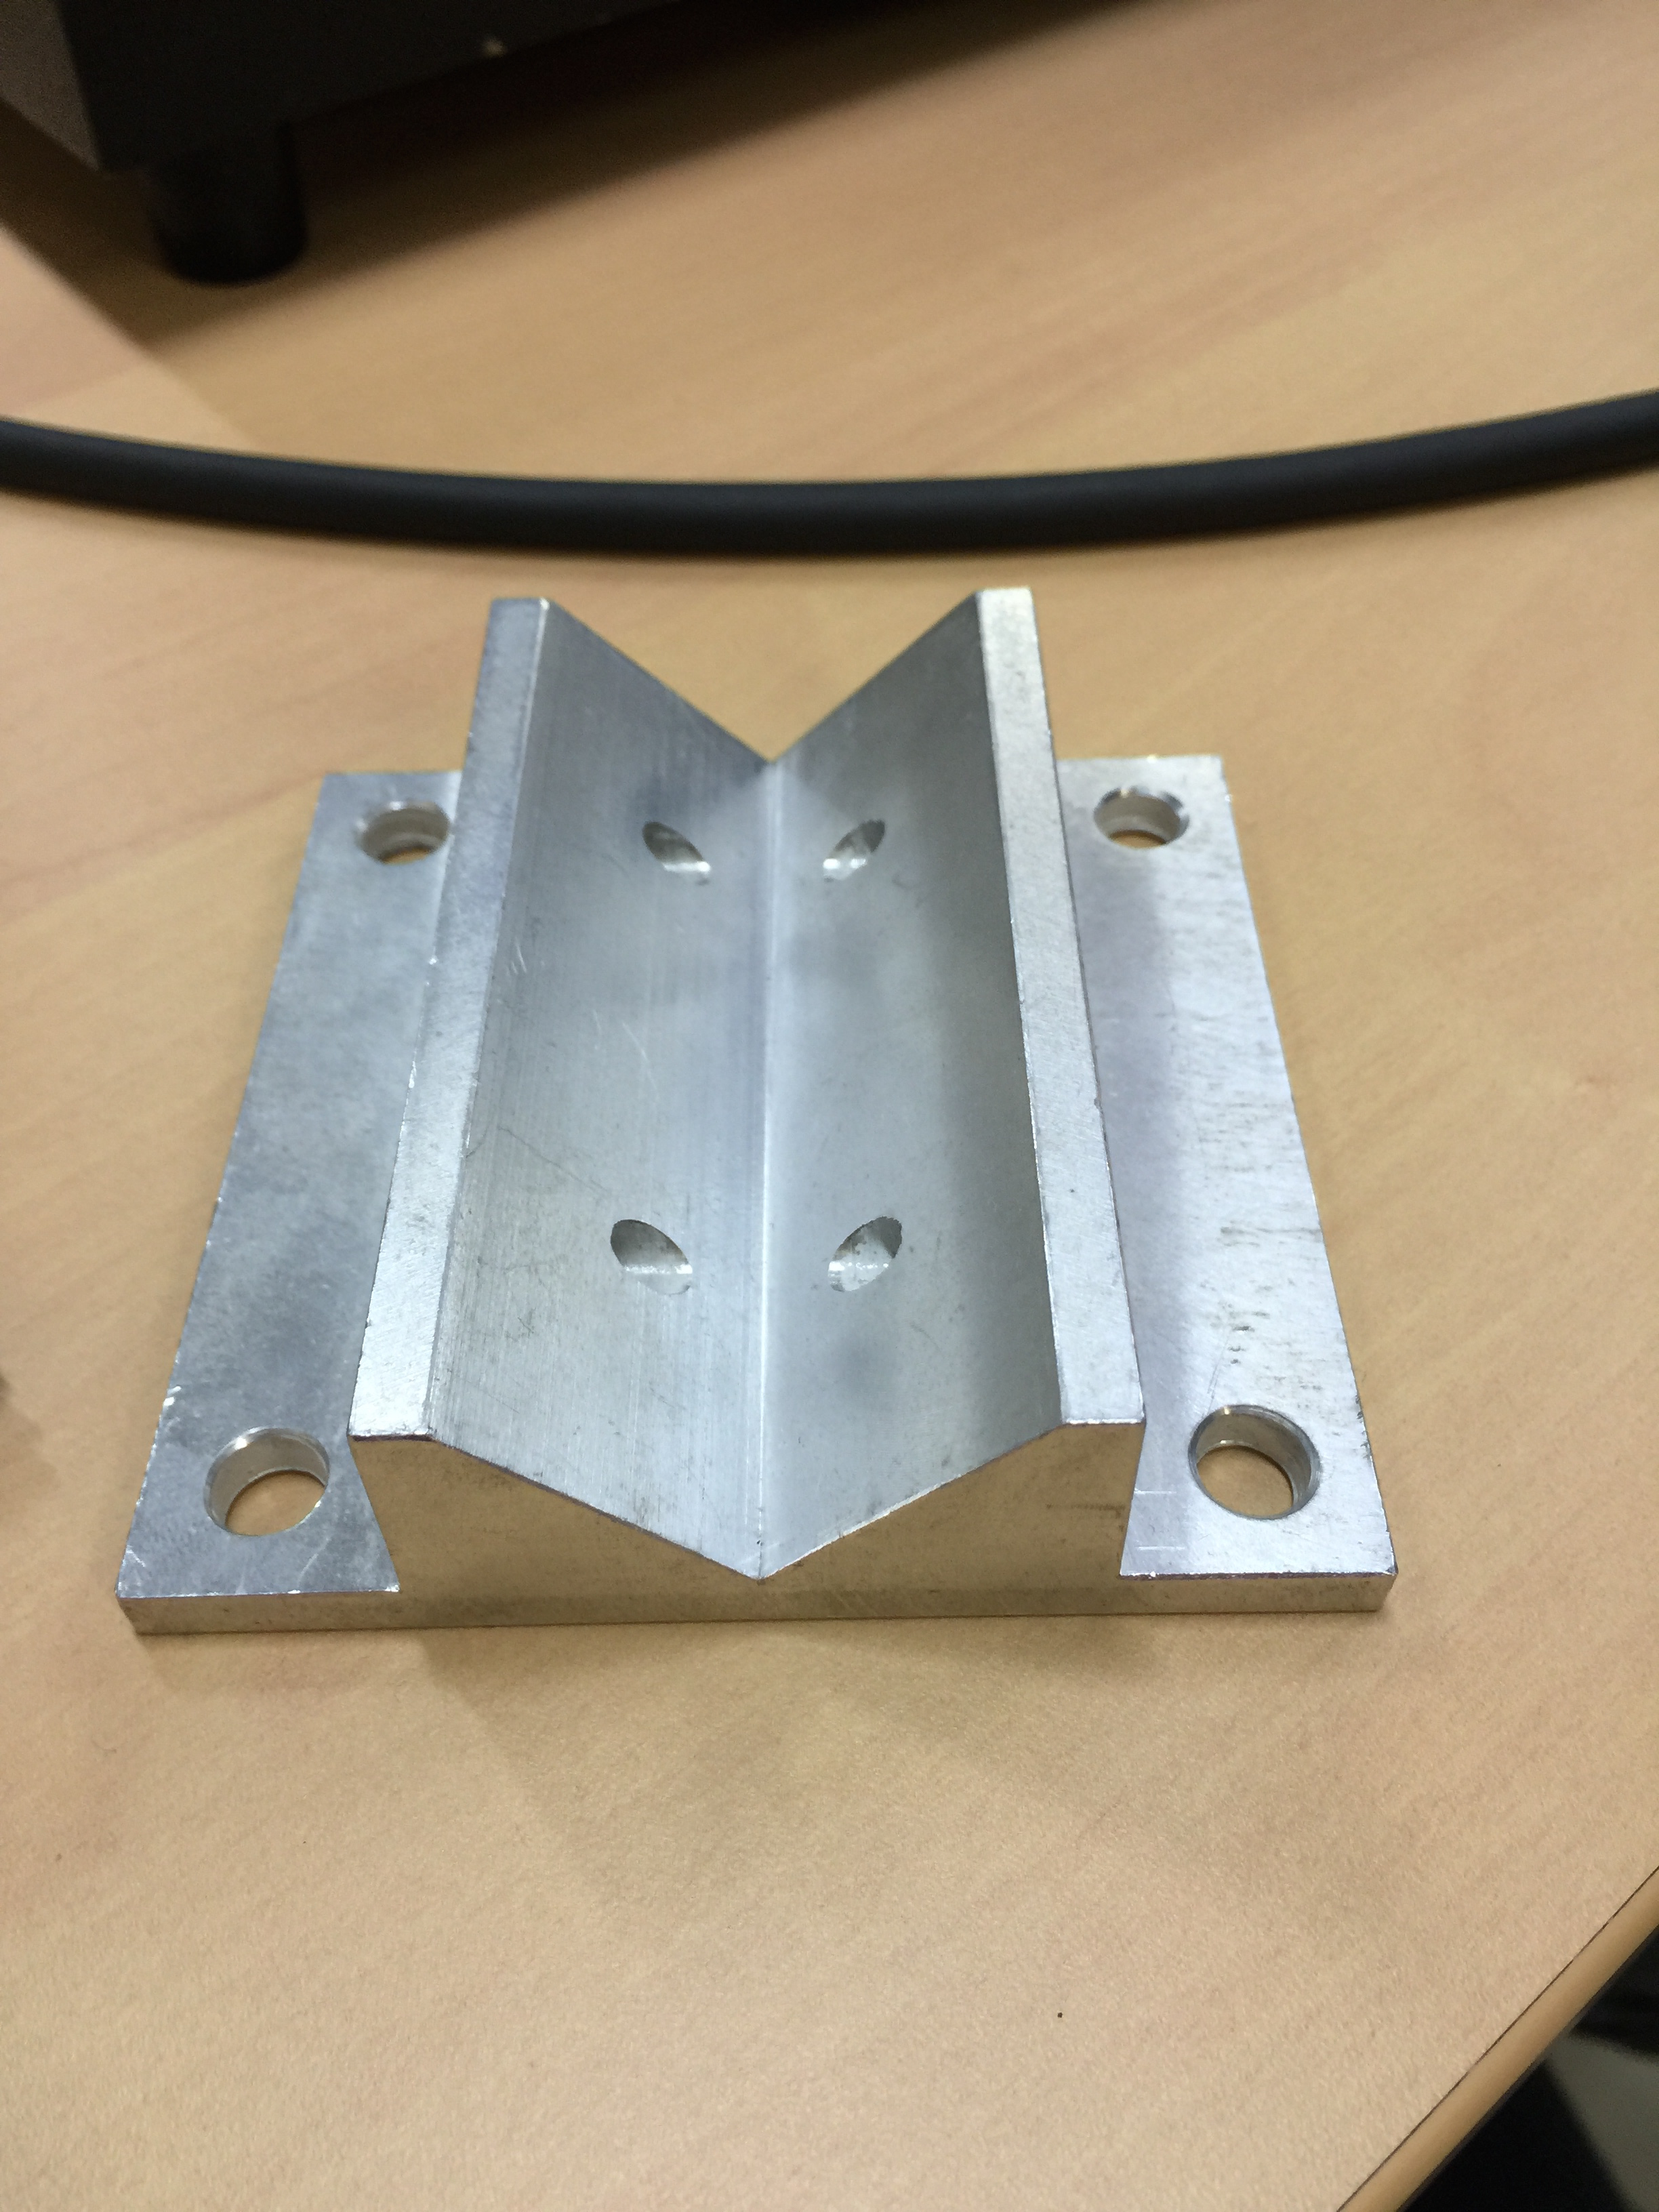
\includegraphics[width=0.6\linewidth]{Lab6/Hole3.JPG}
	}
	\subfigure[Hole in the side]{\label{fig:sixb}
	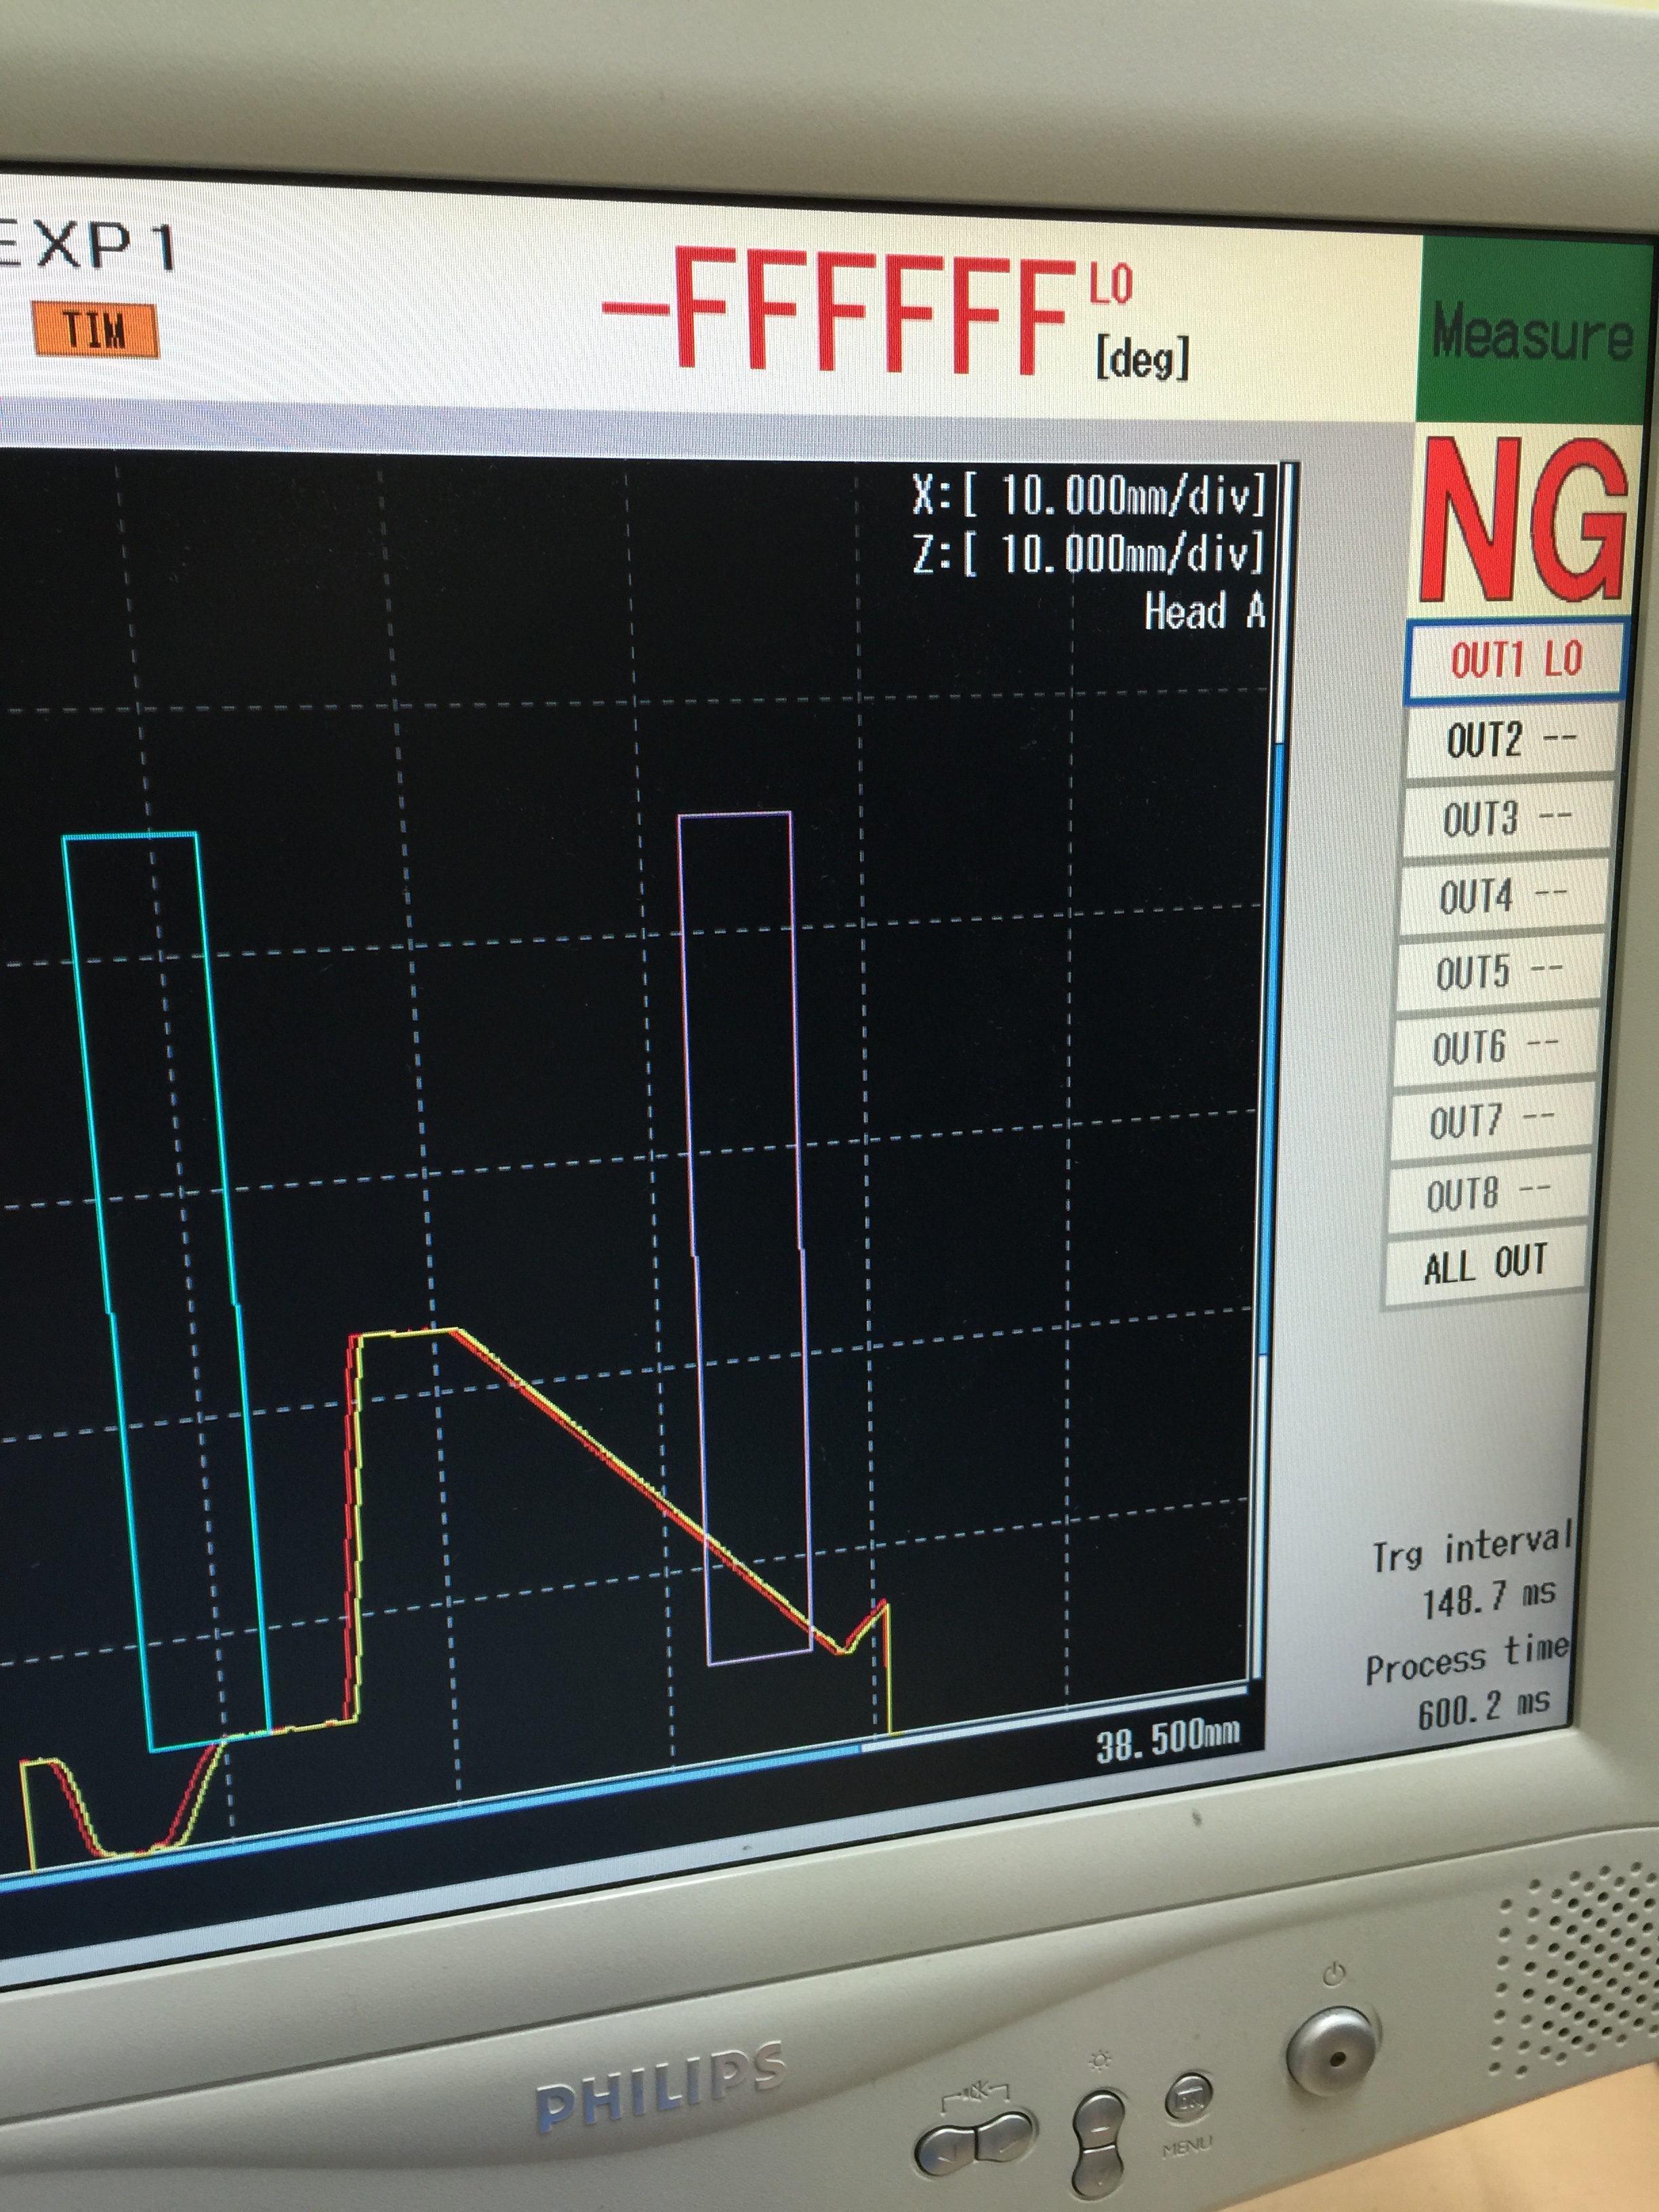
\includegraphics[width=0.45\linewidth]{Lab6/Hole1.JPG}
	}
	\subfigure[Hole in the planes]{\label{fig:sixc}
	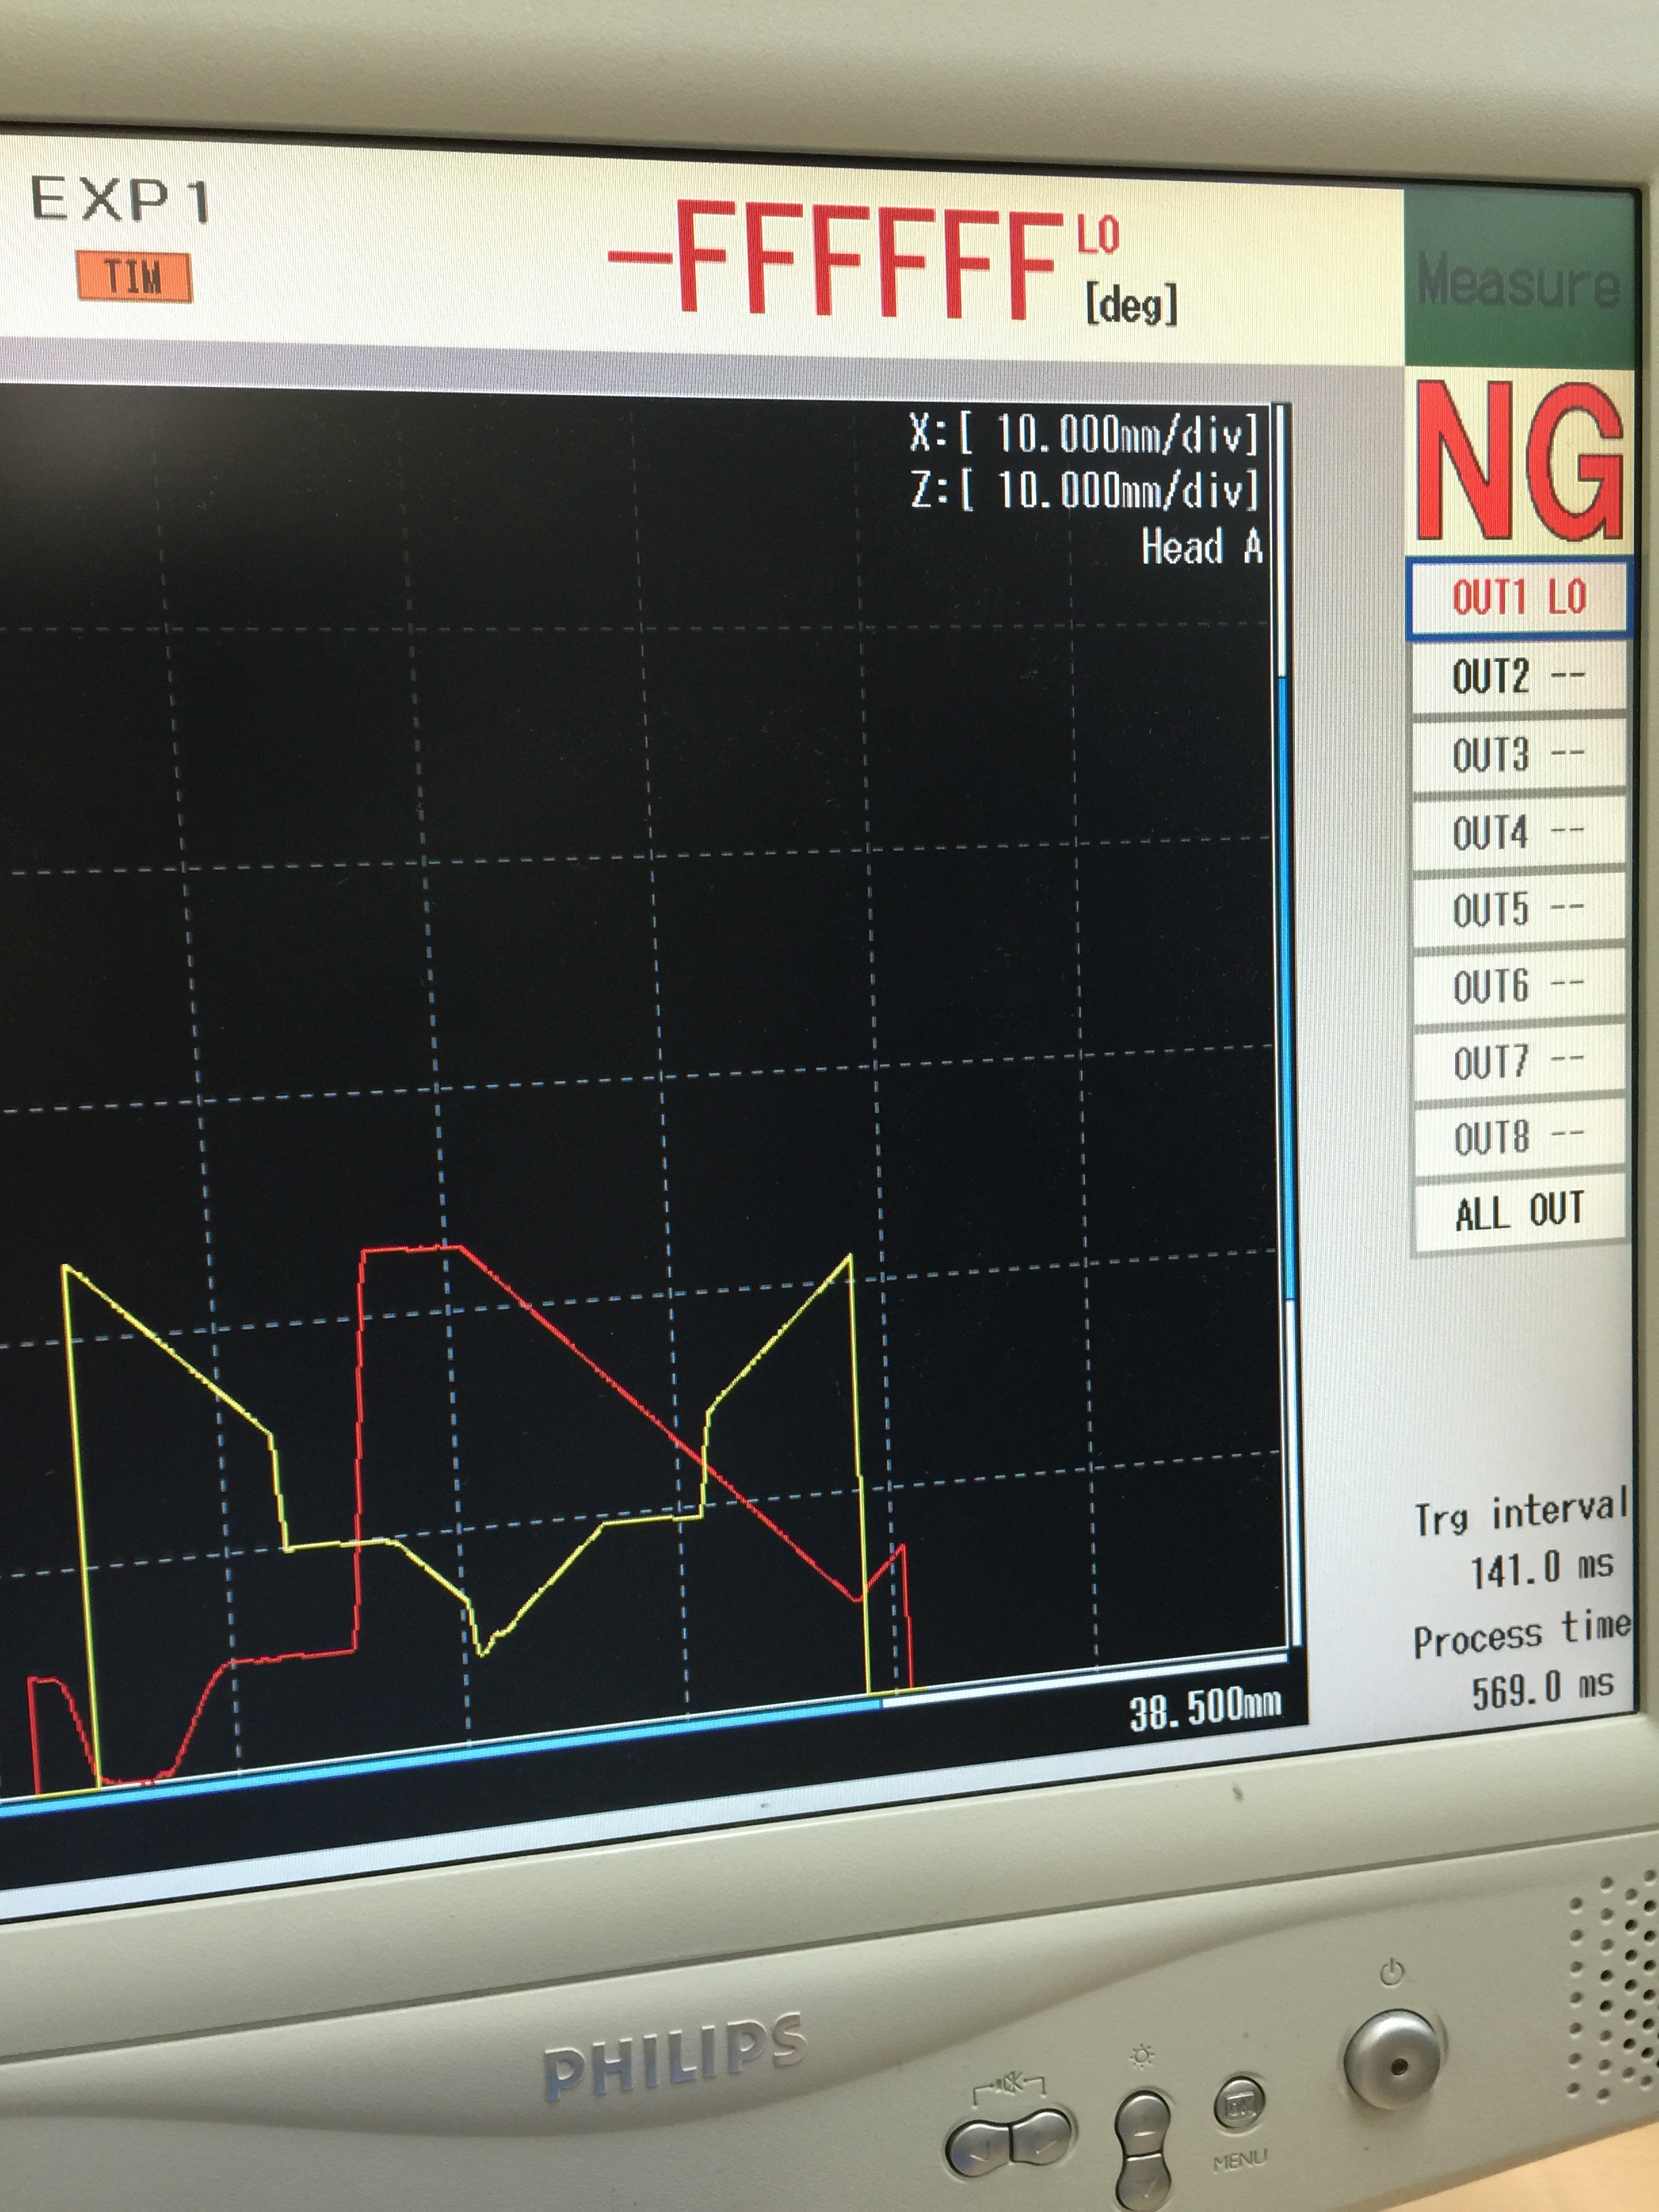
\includegraphics[width=0.45\linewidth]{Lab6/Hole2.JPG}
	}
	\caption{Hole detection}
	\label{fig:six}
\end{figure}


\section*{Conclusion}


\section*{References}

{[}1{]} - https://en.wikipedia.org/wiki/Digital\_camera
\\
{[}2{]} - http://www.baslerweb.com/en/products/line-scan-cameras
\end{document}
